\documentclass[10pt]{article}
\usepackage{tmlr}

% Optional math commands from standard notation
\input{math_commands.tex}

% Required packages
\usepackage[utf8]{inputenc}
\usepackage{amsmath,amssymb,amsfonts,amsthm}
\usepackage{booktabs}
\usepackage{graphicx}
\usepackage{subcaption}
\usepackage{xurl}
\usepackage{hyperref}
\usepackage{microtype}
\usepackage{xcolor}
\usepackage{array}
\usepackage{tabularx}
\usepackage{float}

% Hyperref setup
\hypersetup{
    colorlinks=true,
    linkcolor=blue!70!black,
    citecolor=blue!70!black,
    urlcolor=blue!70!black
}

\title{Candidate Order Instability in Non-Autoregressive\\Multi-Candidate Transformers\thanks{LLM assistance disclosure: During the preparation of this manuscript, the authors utilized large language model assistants solely for drafting suggestions, style refinements, literature query organization, and code formatting. All experimental design, empirical measurements, mathematical proofs, interpretations, and conclusions were independently conducted, rigorously verified, and finalized by the authors, who take full scholarly responsibility for the integrity of this work.}}

% Author and affiliation block suppressed for double-blind review
\author{\name Anonymous Authors \email anonymous@domain.org \\
      \addr Anonymous Institution}

\def\month{MM}
\def\year{YYYY}
\def\openreview{\url{https://openreview.net/forum?id=XXXX}}

\begin{document}

\maketitle

\begin{abstract}
Candidate choices in classification form an unordered set, yet transformer classifiers frequently serialize options into sequential text. We evaluate candidate presentation order in non-autoregressive multi-candidate transformers (\nolinkurl{convaiinnovations/laya}), which score all choices in a single bidirectional pass via delimiter marker representations. Using the Banking77 benchmark under a strictly nested distractor protocol ($K \in \{5, 10, 20, 40, 77\}$) across $N=120$ intent-stratified queries, we observe that pairwise argmax decision instability ($\mathrm{FR}_{\mathrm{top1}}$) increases from $5.70\%$ [3.1\%, 8.4\%] at $K=5$ to $47.28\%$ [42.8\%, 51.9\%] at $K=77$, accompanied by a $7.5\times$ expansion in candidate logit variance. While canonical alphabetical sorting enforces deterministic repeatability, counterfactual reverse-alphabetical sorting reveals a $55.83\%$ [47.5\%, 65.0\%] disagreement rate at $K=77$, demonstrating that canonicalization conceals rather than eliminates positional bias. Inference-time permutation marginalization suppresses residual flip rate to $25.83\%$ ($M=5$ random) and $16.11\%$ ($M=5$ cyclic shifts), while descriptively reducing Expected Calibration Error from $0.3857$ to $0.0960$. Crucially, under Benjamini-Hochberg False Discovery Rate control ($q=0.05$) across 45 pre-specified paired comparisons, only cyclic shifts at $K=40$ achieve statistically significant accuracy gains ($+9.17$ percentage points, adjusted $p=0.04395$); at $K=77$, accuracy gains fail FDR significance. Furthermore, we document the non-replication of an exploratory $65.0\%$ cyclic accuracy finding, which regressed to $48.06\%$ [39.7\%, 55.6\%] under multi-seed replication ($N=120, S=3$). All artifacts, data, and verification suites are openly archived.
\end{abstract}

\section{Introduction}

In classification, dialogue state tracking, intent routing, and tool selection, a classifier is presented with an input query $q$ and a candidate set $\mathcal{C} = \{c_1, \dots, c_K\}$. In mathematical formulations of classification, $\mathcal{C}$ is an unordered set: the set of choices available to the decision rule does not possess an intrinsic sequence. Consequently, an ideal decision function $f(q, \mathcal{C})$ should be permutation-invariant: for any permutation $\pi \in \mathcal{S}_K$, reordering the candidates prior to presentation should yield identical classifications:
\begin{equation}
f(q, \pi(\mathcal{C})) = f(q, \mathcal{C}).
\end{equation}

In practice, modern transformer-based classifiers often serialize choices into text. In autoregressive language models, choices are presented as prompt lists (e.g., ``Options: (A) ... (B) ...''), which have been repeatedly shown to induce recency, primacy, and option-order biases \citep{liu2024lost, pezeshkpour2024large, zheng2024large}. To achieve low-latency inference in agentic routing and intent classification, non-autoregressive multi-candidate transformers \citep{laya2024} evaluate all $K$ candidates simultaneously within a single bidirectional forward pass. In this architecture, candidate strings are concatenated into a single input sequence separated by candidate-specific marker tokens. The sequence is processed by a bidirectional encoder (e.g., RoBERTa; \citealp{liu2019roberta}), and per-candidate classification logits are extracted by projecting the contextualized marker embeddings through a linear head.

While computationally efficient ($O(1)$ forward passes with respect to $K$), serializing unordered choices into a 1D sequence injects artificial positional relationships. Because full bidirectional self-attention couples every token with all other tokens, the contextualized representation of candidate marker $M_k$ is influenced by its absolute position, its relative distance from query tokens, and the semantic identities of its immediate sequence neighbors.

This empirical investigation addresses the question: \textit{Does candidate presentation order act as a hidden nuisance variable in non-autoregressive multi-candidate transformer decision architectures, and how does this sensitivity scale with candidate cardinality $K$?}

To answer this question rigorously, we perform a controlled empirical study using the Banking77 benchmark \citep{casanueva2020efficient} on the open-source \nolinkurl{convaiinnovations/laya} model checkpoint. Our experimental contributions and findings are scoped as follows:
\begin{enumerate}
    \item \textbf{Controlled Distractor Nesting Protocol:} We design a strictly nested candidate-subsampling protocol ($K_5 \subset K_{10} \subset K_{20} \subset K_{40} \subset K_{77}$) over $N=120$ test queries stratified across all 77 intent classes, ensuring that cardinality comparisons are not confounded by stochastic distractor sampling.
    \item \textbf{Order Sensitivity Scaling:} Holding query and candidate sets fixed, random permutations induce an argmax decision flip rate ($\mathrm{FR}_{\mathrm{top1}}$) that increases from $5.70\%$ [3.1\%, 8.4\%] at $K=5$ to $47.28\%$ [42.8\%, 51.9\%] at $K=77$. Cross-permutation candidate logit variance expands by $7.5\times$ ($8.40 \to 63.34$).
    \item \textbf{The Canonicalization Fallacy:} Canonical alphabetical sorting eliminates run-to-run prediction variance ($\mathrm{FR}_{\mathrm{top1}} \equiv 0.0\%$), but counterfactual reverse-alphabetical sorting ($Z \to A$) induces a $55.83\%$ [47.5\%, 65.0\%] disagreement rate at $K=77$. Deterministic serialization locks in exposure bias rather than removing order sensitivity.
    \item \textbf{Inference-Time Order Marginalization:} Without modifying model weights, averaging probability vectors over $M \in \{1, 2, 3, 5\}$ permutations reduces residual decision instability. At $K=77$, random marginalization suppresses residual flip rate to $25.83\%$ ($M=5$), while orthogonal cyclic shifts achieve $16.11\%$ residual flip rate at equal compute.
    \item \textbf{Rigorous Statistical Analysis \& Negative Result:} Across 45 pre-specified paired comparisons controlled under Benjamini-Hochberg False Discovery Rate ($q=0.05$), only one method achieves statistically significant accuracy gains: cyclic shifts at $K=40$ ($+9.17$ percentage points, adjusted $p=0.04395$). At $K=77$, accuracy gains fail FDR significance. Furthermore, we document the non-replication of an exploratory $65.0\%$ accuracy finding, which regressed to $48.06\%$ under pre-specified multi-seed replication.
\end{enumerate}

\section{Related Work}

\subsection{Permutation-Invariant Learning on Sets}
In mathematical formulations of set processing and classification, an input candidate set $\mathcal{X} = \{x_1, \dots, x_K\}$ constitutes an unordered collection of elements. A set function $f: 2^{\mathcal{X}} \to \mathbb{R}^d$ is defined as permutation-invariant if for any permutation $\pi \in \mathcal{S}_K$, $f(\pi(\mathcal{X})) = f(\mathcal{X})$, and permutation-equivariant if $f(\pi(\mathcal{X})) = \pi(f(\mathcal{X}))$.

Foundational principles of deep learning over sets established by \citet{zaheer2017deep} (Deep Sets) establish that any continuous permutation-invariant function acting on countable sets can be decomposed into the canonical form $\rho\left( \sum_{x \in \mathcal{X}} \phi(x) \right)$, where $\phi$ maps instances independently to a latent representation space and $\rho$ applies non-linear transformations subsequent to a symmetric pooling operator (e.g., sum, mean, or max). \citet{lee2019set} extended this framework to model higher-order pairwise and subset interactions using attention mechanisms via the Set Transformer, which employs multi-head attention without positional encodings (through Induced Set Attention Blocks and Pooling by Multihead Attention) to enforce strict permutation equivariance and invariance by construction.

A fundamental distinction must be maintained between three paradigms: (i) a mathematical set function where inputs inherently lack sequential ordering, (ii) permutation-invariant architectures (e.g., Deep Sets and Set Transformer) that structurally enforce invariance by construction, and (iii) a sequence encoder that processes set elements through an ordered 1D serialization. The architecture evaluated in this work (\nolinkurl{convaiinnovations/laya}; \citealp{laya2024}) belongs to the third paradigm. Rather than pooling independent instance projections, it serializes candidate elements into a single prompt string separated by delimiter markers. Consequently, the architecture trades architectural permutation invariance for cross-candidate self-attention context, inherently coupling candidate representations to sequential coordinates.

\subsection{Transformers and Positional Information}
The standard transformer architecture \citep{vaswani2017attention} relies on Scaled Dot-Product Attention, which is fundamentally permutation-equivariant over unordered sets of input tokens in the absence of positional encodings. To enable transformers to parse the syntax and word order of natural language, sequence position information is deliberately introduced. In the original formulation \citep{vaswani2017attention}, sinusoidal positional embeddings were added to token embeddings, whereas modern pretrained bidirectional encoders such as BERT and RoBERTa \citep{liu2019roberta} employ learned absolute positional embeddings.

Subsequent architectural developments introduced relative positional representations \citep{shaw2018self}, rotary position embeddings (RoPE; \citealp{su2024roformer}), and linear attention biases (ALiBi; \citealp{press2022alibi}), which condition attention scores directly on relative token displacements $|i - j|$ rather than absolute sequence indices. As systematically reviewed by \citet{dufter2022position}, positional representations fundamentally shape self-attention dynamics: they bias attention distributions toward local sequence neighborhoods, alter token representation geometry across successive layers, and cause self-attention entropy to redistribute as sequence length scales.

This literature provides the core mechanistic motivation for our investigation: because positional encodings inject non-uniform spatial inductive biases, serializing unordered candidates into a 1D sequence inevitably exposes each candidate marker to position-dependent representational shifts. However, positional encoding literature alone does not establish or prove the presence of candidate-order instability in multi-candidate concatenation architectures; empirical evaluation is necessary to measure its real-world magnitude.

\subsection{Order Sensitivity in Language Models}
Order-dependent sensitivity has been widely documented in recent empirical studies of pretrained language models, spanning three distinct phenomena:
\begin{enumerate}
    \item \textbf{Few-shot prompt demonstration ordering:} \citet{lu2022fantastically} observed that the presentation order of in-context exemplars in few-shot prompts dramatically impacts autoregressive language model accuracy, causing performance to swing between near-chance accuracy and peak benchmark accuracy across permutations of the exact same demonstration set. \citet{zhao2021calibrate} similarly identified substantial majority-label, recency, and common-token biases in prompt-based classification, introducing test-time affine calibration of output logits.
    \item \textbf{Context ordering and positional bias:} In document retrieval and question answering over long sequences, \citet{liu2024lost} demonstrated the ``lost-in-the-middle'' phenomenon: language models retrieve information effectively when relevant context is placed at the extreme beginning or end of the input sequence, but experience severe performance degradation when relevant passages reside in the interior.
    \item \textbf{Option order bias in multiple-choice selection:} When multiple-choice questions are presented to large language models with letter-labeled options (e.g., A, B, C, D), \citet{pezeshkpour2024large} and \citet{zheng2024large} demonstrated that models exhibit strong selection biases toward specific option positions or identifiers, frequently flipping their selected choice when options are permuted.
\end{enumerate}

To properly contextualize the present study, it is critical to distinguish these prior phenomena from the problem addressed here. We do not evaluate prompt demonstration ordering in few-shot in-context learning \citep{lu2022fantastically}, nor natural language token order in autoregressive generation, nor letter-associated choice options evaluated via next-token generation probabilities \citep{pezeshkpour2024large, zheng2024large}. Instead, our study focuses on candidate ordering in a non-autoregressive, encoder-based discriminative architecture: all $K$ candidates are concatenated into a single bidirectional sequence with delimiter markers, and classification logits are simultaneously extracted from marker embeddings via a shared linear head.

\subsection{Intent Classification and Candidate Selection}
Intent classification serves as a cornerstone task in conversational AI, dialogue state tracking, and agentic tool routing, where user queries must be matched against pre-defined intent categories. The Banking77 benchmark \citep{casanueva2020efficient} provides an authoritative, fine-grained evaluation suite comprising 13,083 customer service utterances spanning 77 intent classes. Its high semantic density and fine granularity---distinguishing between closely related categories such as \texttt{card\_arrival}, \texttt{card\_linking}, and \texttt{card\_delivery\_estimate}---provide a realistic, challenging testbed where distractors exhibit strong semantic overlap.

Multi-candidate selection in conversational systems has traditionally relied on two architectural paradigms:
\begin{itemize}
    \item \textbf{Dual-encoders (Bi-encoders):} Queries and candidate labels are encoded into independent dense representations, and similarity is scored via dot-product or cosine distance \citep{casanueva2020efficient}. Dual-encoders are strictly permutation-invariant with respect to candidate presentation and achieve $O(1)$ query forward passes with pre-indexed candidates. However, they lack cross-attention between candidates and the query during encoding, limiting discriminative capacity.
    \item \textbf{Cross-encoders:} The query and each candidate are concatenated into a single sequence (\texttt{[CLS] q [SEP] c [SEP]}) and processed with full cross-attention \citep{nogueira2019passage}. While cross-encoders achieve high accuracy by modeling fine-grained query-candidate interactions, scoring $K$ candidates requires $K$ separate forward passes ($O(K)$ complexity), creating prohibitive latency overheads in real-time agentic routing.
    \item \textbf{Poly-encoders:} \citet{humeau2020polyencoders} bridge this trade-off by extracting multiple contextual query embeddings and attending over candidate encodings, but preserve separate candidate representations.
\end{itemize}
The non-autoregressive multi-candidate architecture (\nolinkurl{convaiinnovations/laya}; \citealp{laya2024}) attempts to overcome the $O(K)$ computational barrier of cross-encoders while retaining cross-attention by packing all $K$ candidates into a single sequence separated by reserved delimiter tokens. This design achieves $O(1)$ forward passes with full bidirectional cross-candidate attention, but introduces sequence serialization order as an unmodelled confounding variable.

\subsection{Calibration and Inference-Time Marginalization}
\paragraph{Confidence Calibration.} In automated decision routing and tool invocation, predicted confidence scores govern critical control decisions: whether to execute an action autonomously, prompt the user for confirmation, or route to a human operator. A classifier is well-calibrated when predicted probabilities correspond to empirical accuracy: $\mathbb{P}(\hat{y} = y \mid \hat{p} = p) = p$ \citep{guo2017calibration}. Expected Calibration Error (ECE; \citealp{naeini2015obtaining, nixon2019measuring}) quantifies calibration mismatch by partitioning predictions into discrete confidence bins. Deep neural networks, particularly modern transformer architectures, are well known to produce poorly calibrated, overconfident posterior distributions \citep{guo2017calibration}. In this study, we measure whether candidate order permutation and ensemble marginalization affect empirical calibration, evaluating ECE through clustered bootstrap distributions.

\paragraph{Ensembling and Test-Time Augmentation.} Aggregating predictions across perturbed inputs has deep roots in statistical learning and uncertainty estimation:
\begin{itemize}
    \item \textbf{Deep Ensembles:} \citet{lakshminarayanan2017simple} established that ensembling independently trained models significantly improves predictive accuracy and uncertainty calibration.
    \item \textbf{Test-Time Augmentation (TTA):} In computer vision, applying stochastic data augmentations (e.g., cropping, scaling, rotation) at test time and averaging predictions provides effective marginalization over nuisance variations, reducing aleatoric uncertainty and boosting accuracy \citep{ayhan2018test, shanmugam2020when}.
    \item \textbf{Self-Consistency in Language Models:} In complex reasoning tasks with generative LLMs, \citet{wang2023selfconsistency} demonstrated that sampling diverse reasoning paths and taking a marginal majority vote yields substantial performance improvements over greedy decoding.
\end{itemize}
Our study introduces an inference-time order-marginalization framework tailored to non-autoregressive multi-candidate encoders. By treating candidate presentation order as an input perturbation, we examine whether averaging predictions over random permutations or structured orthogonal cyclic shifts recovers decision stability and improves calibration without modifying model weights.

\subsection{Positioning of the Present Study: Critical Gap Analysis}
To establish the distinct empirical contribution of this paper, we summarize the relationship between prior work and our investigation:
\begin{enumerate}
    \item Prior work on Deep Sets \citep{zaheer2017deep} and Set Transformers \citep{lee2019set} proves that permutation invariance can be built into architectures, but requires specialized pooling or unpositioned attention. We evaluate whether off-the-shelf bidirectional sequence encoders can achieve operational invariance when candidates are serialized as text.
    \item Positional encoding studies \citep{vaswani2017attention, su2024roformer, dufter2022position} establish that position embeddings shape attention geometry, but do not measure or quantify candidate order instability in multi-candidate discriminators.
    \item Prior empirical NLP work on order sensitivity focused on autoregressive generation \citep{lu2022fantastically, zhao2021calibrate, liu2024lost, pezeshkpour2024large, zheng2024large}. Our work is the first to measure order instability in non-autoregressive encoders that evaluate all $K$ candidates simultaneously via delimiter marker representations.
    \item While previous intent classification benchmarks \citep{casanueva2020efficient} evaluated bi-encoders and cross-encoders, they treated candidate sets as fixed indices. We study the internal sequence dynamics when candidate sets scale from $K=5$ to $K=77$.
    \item Test-time augmentation \citep{ayhan2018test, shanmugam2020when} has primarily targeted image transformations. We apply test-time input perturbation to discrete candidate permutations in text serialization.
    \item Many engineering pipelines employ alphabetical sorting under the assumption that deterministic repeatability is equivalent to permutation invariance. We show that alphabetical sorting conceals a substantial counterfactual exposure bias ($55.83\%$ disagreement under reverse sorting).
    \item Finally, we demonstrate the necessity of multiple testing corrections in multi-candidate evaluations: while multiple interventions appear promising in unadjusted tests, Benjamini-Hochberg FDR control reveals that only one intervention achieves statistically significant accuracy gains, and multi-seed replication corrects an exploratory $65.0\%$ artifact.
\end{enumerate}

\section{Problem Formulation and Model Architecture}

\subsection{Architectural Mechanism}

The model under evaluation (\nolinkurl{convaiinnovations/laya}) implements a single-pass multi-candidate classification architecture. Given an input query $q$ and candidate intents $\mathcal{C} = \{c_0, c_1, \dots, c_{K-1}\}$, the serialization module serializes the components into a single token sequence:
\begin{equation}
\mathbf{x}(\pi) = \left[ \texttt{[CLS]}, q_1, \dots, q_L, \texttt{[SEP]}, \texttt{[M}_0\texttt{]}, c_{\pi(0)}, \texttt{[M}_1\texttt{]}, c_{\pi(1)}, \dots, \texttt{[M}_{K-1}\texttt{]}, c_{\pi(K-1)}, \texttt{[SEP]} \right]
\end{equation}
where $\texttt{[M}_i\texttt{]}$ denotes a reserved structural marker token, and $\pi \in \mathcal{S}_K$ denotes a candidate permutation.

The serialized sequence $\mathbf{x}(\pi)$ is processed by a bidirectional transformer encoder (RoBERTa backbone with Scaled Dot-Product Attention; \citealp{vaswani2017attention, liu2019roberta}):
\begin{equation}
\mathbf{H} = \text{Encoder}(\mathbf{x}(\pi)) \in \mathbb{R}^{T \times d}.
\end{equation}
Let $\mathbf{h}_{M_k}(\pi) \in \mathbb{R}^d$ denote the final hidden state corresponding to the marker token preceding candidate $c_k$. Per-candidate classification logits are computed via a shared linear projection head $\mathbf{w} \in \mathbb{R}^d$:
\begin{equation}
s(q, c_k; \pi) = \mathbf{w}^\top \mathbf{h}_{M_k}(\pi).
\end{equation}
Class probabilities over the $K$ choices are obtained by applying a softmax over candidate logits:
\begin{equation}
p(c_k \mid q; \pi) = \frac{\exp(s(q, c_k; \pi))}{\sum_{j=0}^{K-1} \exp(s(q, c_j; \pi))}.
\end{equation}
The predicted class is selected via argmax: $\hat{y}(\pi) = \operatorname*{argmax}_{k} s(q, c_k; \pi)$.

\subsection{Theoretical Origin of Order Instability}

In standard multi-head self-attention with learned absolute position embeddings $\mathbf{P} \in \mathbb{R}^{T \times d}$, token representations are given by $\mathbf{z}_i = \mathbf{e}_i + \mathbf{p}_i$. The attention weight between candidate marker $M_k$ and any token $j$ depends directly on their absolute positions:
\begin{equation}
A_{i,j} = \frac{\exp\left( (\mathbf{z}_i \mathbf{W}_Q)(\mathbf{z}_j \mathbf{W}_K)^\top / \sqrt{d_k} \right)}{\sum_{l=1}^T \exp\left( (\mathbf{z}_i \mathbf{W}_Q)(\mathbf{z}_l \mathbf{W}_K)^\top / \sqrt{d_k} \right)}.
\end{equation}
When the permutation $\pi$ changes, three distinct shifts occur:
\begin{enumerate}
    \item \textbf{Position Embedding Shift:} The absolute position of candidate $c_k$ changes from index $i$ to $i'$, replacing $\mathbf{p}_i$ with $\mathbf{p}_{i'}$.
    \item \textbf{Attentional Distance to Query:} The relative distance $|i - j|$ between candidate marker $M_k$ and the query tokens $\{q_1, \dots, q_L\}$ varies across permutations.
    \item \textbf{Local Context Modulation:} The immediate neighbor candidates preceding and following $c_k$ change, altering local key-value aggregations in lower layers.
\end{enumerate}
Consequently, $\mathbf{h}_{M_k}(\pi_1) \neq \mathbf{h}_{M_k}(\pi_2)$, producing varying classification logits $s(q, c_k; \pi_1) \neq s(q, c_k; \pi_2)$ and potentially flipping the top-1 predicted class.

\section{Experimental Setup}

\subsection{Benchmark Dataset and Query Stratification}
We evaluate on the Banking77 benchmark \citep{casanueva2020efficient}, which contains 3,080 test queries across 77 fine-grained banking intent categories. To ensure representative coverage across the full semantic space while maintaining computational feasibility for multi-permutation evaluations, we construct an intent-stratified evaluation sample of $N=120$ unique queries:
\begin{itemize}
    \item All 77 intent classes are guaranteed representation (1 query per class for all 77 classes).
    \item An additional 43 queries are sampled proportionally across frequent classes.
    \item The test query set $\mathcal{Q}$ ($|\mathcal{Q}| = 120$) is held strictly identical across all cardinalities and all evaluated methods.
\end{itemize}

\subsection{Controlled Distractor Nesting Protocol}
To evaluate candidate cardinality scaling without confounding from distractor difficulty, we implement a strictly nested candidate selection hierarchy:
\begin{equation}
\mathcal{C}_5(q) \subset \mathcal{C}_{10}(q) \subset \mathcal{C}_{20}(q) \subset \mathcal{C}_{40}(q) \subset \mathcal{C}_{77}(q) = \mathcal{C}_{\text{all}}.
\end{equation}
For each query $q$ with ground-truth label $y^*$, the candidate set $\mathcal{C}_K(q)$ contains:
\begin{enumerate}
    \item The true ground-truth label $y^* \in \mathcal{C}_K(q)$ for all $K$.
    \item $K-1$ distractor labels selected via deterministic pseudo-random sampling seeded by query ID.
    \item Distractors for smaller $K$ are strictly preserved as subsets of larger $K$ candidate sets.
\end{enumerate}

\subsection{Intervention Methods Evaluated}
We evaluate ten distinct inference methods spanning baselines, canonicalization, and marginalization:
\begin{itemize}
    \item \textbf{B0\_Native:} Single forward pass using default dataset candidate order.
    \item \textbf{B0\_Random:} Single forward pass with uniformly random candidate permutation.
    \item \textbf{B1\_Alpha:} Single forward pass with candidates sorted alphabetically ($A \to Z$).
    \item \textbf{B1\_ReverseAlpha:} Counterfactual reverse alphabetical candidate order ($Z \to A$).
    \item \textbf{Rand\_Marg\_M\{2,3,5\}:} Probability averaging over $M \in \{2, 3, 5\}$ independent random candidate permutations: $\bar{\mathbf{p}} = \frac{1}{M}\sum_{m=1}^M \mathbf{p}(\pi_m)$.
    \item \textbf{B2\_Cyclic\_M\{2,3,5\}:} Probability averaging over $M$ deterministic orthogonal cyclic shifts: $\pi_m(i) = (i + m \cdot \lfloor K/M \rfloor) \pmod K$.
\end{itemize}

\subsection{Multi-Seed Replication at Maximum Cardinality (\texorpdfstring{$K=77$}{K=77})}
To prevent anchoring bias and eliminate exploratory sampling artifacts, all evaluations at $K=77$ are executed across $S=3$ independently seeded base candidate sequences: (i) `alphabetical', (ii) \texttt{seed\_7701}, and (iii) \texttt{seed\_7702}. Reported metrics at $K=77$ represent pooled expectations across all $S=3$ runs ($N \times S = 360$ evaluations per method).

\section{Metrics and Statistical Analysis}

\subsection{Mathematical Definitions}

\paragraph{1. Pairwise Top-1 Flip Rate ($\mathrm{FR}_{\mathrm{top1}}$).}
For a given query $q$ and candidate set $\mathcal{C}$, the pairwise argmax decision flip rate measures the probability that two independent random permutations yield conflicting predictions:
\begin{equation}
\mathrm{FR}_{\mathrm{top1}}(q, \mathcal{C}) = \mathbb{E}_{\pi_1, \pi_2 \sim \mathcal{S}_K} \left[ \mathbf{1}\left( \operatorname*{argmax}_{c \in \mathcal{C}} s(q, c; \pi_1) \neq \operatorname*{argmax}_{c \in \mathcal{C}} s(q, c; \pi_2) \right) \right].
\end{equation}
For $P=10$ random permutations per query, $\mathrm{FR}_{\mathrm{top1}}(q)$ is estimated as a degree-2 $U$-statistic over all $\binom{10}{2} = 45$ pairwise permutation comparisons. The independent statistical sampling unit is strictly the query ID ($N=120$).

\paragraph{2. Cross-Canonical Flip Rate ($\mathrm{CrossCanonicalFlip}$).}
For deterministic alphabetical sorting (`B1\_Alpha'), within-method permutation instability is identically zero ($\mathrm{FR}_{\mathrm{top1}} \equiv 0.0\%$) because repeating identical input strings yields deterministic model outputs. To measure true underlying positional bias, we define the cross-canonical disagreement rate between alphabetical and reverse-alphabetical orderings:
\begin{equation}
\mathrm{CrossCanonicalFlip}(q, \mathcal{C}) = \mathbf{1}\left( \operatorname*{argmax}_{c \in \mathcal{C}} s(q, c; \pi_{\alpha}) \neq \operatorname*{argmax}_{c \in \mathcal{C}} s(q, c; \pi_{\mathrm{rev}\text{-}\alpha}) \right).
\end{equation}
$\mathrm{FR}_{\mathrm{top1}}$ and $\mathrm{CrossCanonicalFlip}$ are maintained as separate metrics throughout our analysis.

\paragraph{3. Residual Ensemble Flip Rate ($\mathrm{ResFlip}_M$).}
To measure residual instability after marginalizing over $M$ permutations, we evaluate the discordance between two non-overlapping $M$-pass ensembles:
\begin{equation}
\mathrm{ResFlip}_M(q) = \mathbf{1}\left( \operatorname*{argmax}_{c} \frac{1}{M}\sum_{m=1}^M p(c; \pi_m) \neq \operatorname*{argmax}_{c} \frac{1}{M}\sum_{m=M+1}^{2M} p(c; \pi_m) \right).
\end{equation}

\paragraph{4. Expected Calibration Error (ECE).}
Predictions are partitioned into $B=15$ equally spaced confidence bins $I_b = (\frac{b-1}{B}, \frac{b}{B}]$. Binned calibration error is calculated directly over the model's calibrated probability outputs \citep{guo2017calibration, naeini2015obtaining, nixon2019measuring}:
\begin{equation}
\mathrm{ECE} = \sum_{b=1}^B \frac{|I_b|}{N} \left| \operatorname{acc}(I_b) - \operatorname{conf}(I_b) \right|.
\end{equation}

\paragraph{5. Normalized Kendall's Tau Distance ($\tau_{\mathrm{norm}}$).}
The fraction of discordant candidate pairs between two ranking vectors over $K$ choices \citep{kendall1938new}:
\begin{equation}
\tau_{\mathrm{norm}}(s_a, s_b) = \frac{1}{\binom{K}{2}} \sum_{1 \le i < j \le K} \mathbf{1}\left( (s_a[i] - s_a[j])(s_b[i] - s_b[j]) < 0 \right).
\end{equation}

\subsection{Statistical Protocol}
\begin{itemize}
    \item \textbf{Query-Level Clustered Bootstrap:} All 95\% confidence intervals are generated using $B=1,000$ query-level bootstrap resamples with replacement ($N=120$) \citep{efron1993introduction}. For ECE, the full 15-bin formula is re-evaluated on each bootstrap sample to produce valid empirical percentiles.
    \item \textbf{Paired Hypothesis Tests:} Differences in top-1 accuracy between interventions and `B0\_Native' are evaluated using exact two-sided McNemar tests on discordant classification pairs \citep{mcnemar1947note}.
    \item \textbf{Multiple Testing Correction:} To guard against false positive discoveries across exploratory comparisons, we apply Benjamini-Hochberg False Discovery Rate (FDR) control at $q=0.05$ across all 45 pre-specified hypotheses ($5 \text{ cardinalities} \times 9 \text{ intervention methods}$) \citep{benjamini1995controlling}.
\end{itemize}

\section{Results}

\begin{table*}[t]
\centering
\small
\caption{\textbf{Candidate Cardinality Scaling Results.} Evaluated across $N=120$ intent-stratified queries. $\mathrm{FR}_{\mathrm{top1}}$ is the within-method pairwise argmax flip rate. Cross-Flip measures disagreement between alphabetical and reverse-alphabetical sorting. P-values reflect Benjamini-Hochberg FDR adjustments across 45 paired McNemar tests against `B0\_Native'.}
\label{tab:main_results}
\resizebox{\textwidth}{!}{%
\begin{tabular}{r r l c c c c r c}
\toprule
$K$ & Chance & Method & Accuracy [95\% CI] & ECE [95\% CI] & $\text{FR}_{\text{top1}}$ [95\% CI] & Cross-Flip & Latency & FDR Sig \\
\midrule
5  & 20.0\% & \textbf{B0\_Native} & 0.942 [0.89, 0.98] & 0.089 [0.06, 0.16] & 0.000 [0.00, 0.00] & -- & 23.4 ms & No \\
5  & 20.0\% & \textbf{B0\_Random} & 0.939 [0.89, 0.98] & 0.076 [0.05, 0.14] & 0.057 [0.03, 0.08] & -- & 23.4 ms & No \\
5  & 20.0\% & \textbf{B1\_Alpha}  & 0.925 [0.87, 0.97] & 0.085 [0.06, 0.15] & 0.000 [0.00, 0.00] & 0.033 & 23.4 ms & No \\
5  & 20.0\% & \textbf{Rand\_Marg\_M5} & 0.942 [0.90, 0.98] & 0.079 [0.05, 0.14] & 0.008 [0.00, 0.03] & -- & 117.0 ms & No \\
5  & 20.0\% & \textbf{B2\_Cyclic\_M5} & 0.942 [0.89, 0.98] & 0.080 [0.05, 0.14] & 0.000 [0.00, 0.00] & -- & 117.0 ms & No \\
\midrule
10 & 10.0\% & \textbf{B0\_Native} & 0.900 [0.84, 0.95] & 0.089 [0.06, 0.17] & 0.000 [0.00, 0.00] & -- & 40.5 ms & No \\
10 & 10.0\% & \textbf{B0\_Random} & 0.908 [0.85, 0.95] & 0.085 [0.06, 0.15] & 0.064 [0.04, 0.09] & -- & 40.5 ms & No \\
10 & 10.0\% & \textbf{B1\_Alpha}  & 0.900 [0.84, 0.95] & 0.087 [0.06, 0.16] & 0.000 [0.00, 0.00] & 0.050 & 40.5 ms & No \\
10 & 10.0\% & \textbf{Rand\_Marg\_M5} & 0.908 [0.85, 0.96] & 0.072 [0.05, 0.13] & 0.025 [0.00, 0.06] & -- & 202.5 ms & No \\
10 & 10.0\% & \textbf{B2\_Cyclic\_M5} & 0.908 [0.85, 0.95] & 0.080 [0.05, 0.15] & 0.008 [0.00, 0.03] & -- & 202.5 ms & No \\
\midrule
20 & 5.0\% & \textbf{B0\_Native} & 0.750 [0.67, 0.83] & 0.197 [0.15, 0.28] & 0.000 [0.00, 0.00] & -- & 97.4 ms & No \\
20 & 5.0\% & \textbf{B0\_Random} & 0.772 [0.69, 0.84] & 0.187 [0.14, 0.27] & 0.120 [0.08, 0.16] & -- & 97.4 ms & No \\
20 & 5.0\% & \textbf{B1\_Alpha}  & 0.775 [0.70, 0.85] & 0.168 [0.12, 0.25] & 0.000 [0.00, 0.00] & 0.117 & 97.4 ms & No \\
20 & 5.0\% & \textbf{Rand\_Marg\_M5} & 0.800 [0.72, 0.87] & 0.138 [0.10, 0.22] & 0.050 [0.02, 0.09] & -- & 486.8 ms & No \\
20 & 5.0\% & \textbf{B2\_Cyclic\_M5} & 0.792 [0.72, 0.87] & 0.107 [0.08, 0.19] & 0.033 [0.01, 0.07] & -- & 486.8 ms & No \\
\midrule
40 & 2.5\% & \textbf{B0\_Native} & 0.617 [0.53, 0.71] & 0.265 [0.21, 0.36] & 0.000 [0.00, 0.00] & -- & 146.1 ms & No \\
40 & 2.5\% & \textbf{B0\_Random} & 0.650 [0.56, 0.73] & 0.267 [0.21, 0.36] & 0.221 [0.18, 0.27] & -- & 146.1 ms & No \\
40 & 2.5\% & \textbf{B1\_Alpha}  & 0.692 [0.61, 0.77] & 0.212 [0.16, 0.30] & 0.000 [0.00, 0.00] & 0.167 & 146.1 ms & No \\
40 & 2.5\% & \textbf{Rand\_Marg\_M5} & 0.700 [0.62, 0.78] & 0.180 [0.14, 0.27] & 0.117 [0.06, 0.18] & -- & 730.4 ms & No \\
40 & 2.5\% & \textbf{B2\_Cyclic\_M5} & \textbf{0.708 [0.62, 0.79]} & \textbf{0.172 [0.13, 0.26]} & \textbf{0.050 [0.02, 0.09]} & -- & \textbf{730.4 ms} & \textbf{Yes} ($*$) \\
\midrule
77 & 1.3\% & \textbf{B0\_Native} & 0.422 [0.34, 0.50] & 0.370 [0.30, 0.45] & 0.000 [0.00, 0.00] & -- & 224.7 ms & No \\
77 & 1.3\% & \textbf{B0\_Random} & 0.436 [0.36, 0.51] & 0.386 [0.31, 0.47] & 0.473 [0.43, 0.52] & -- & 224.7 ms & No \\
77 & 1.3\% & \textbf{B1\_Alpha}  & 0.492 [0.40, 0.58] & 0.334 [0.27, 0.43] & 0.000 [0.00, 0.00] & 0.558 & 224.7 ms & No \\
77 & 1.3\% & \textbf{Rand\_Marg\_M5} & 0.550 [0.47, 0.62] & 0.096 [0.09, 0.20] & 0.258 [0.20, 0.32] & -- & 1123.4 ms & No \\
77 & 1.3\% & \textbf{B2\_Cyclic\_M5} & 0.497 [0.42, 0.57] & 0.162 [0.13, 0.26] & 0.161 [0.12, 0.21] & -- & 1123.4 ms & No \\
\bottomrule
\end{tabular}%
}
\end{table*}

\subsection{Cardinality Scaling of Order Instability}

As reported in Table~\ref{tab:main_results} and illustrated in Figure~\ref{fig:cardinality_instability}, candidate presentation order induces measurable decision instability across all evaluated cardinalities. When the candidate set $\mathcal{C}$ and query $q$ are held strictly constant, the pairwise argmax flip rate $\mathrm{FR}_{\mathrm{top1}}$ increases strongly from $5.70\%$ [3.1\%, 8.4\%] at $K=5$ to $47.28\%$ [42.8\%, 51.9\%] at $K=77$. At $K=77$, nearly half of all random permutation pairs yield discordant top-1 predictions for the exact same input query.

\begin{figure}[H]
\centering
\begin{subfigure}[b]{0.48\textwidth}
    \centering
    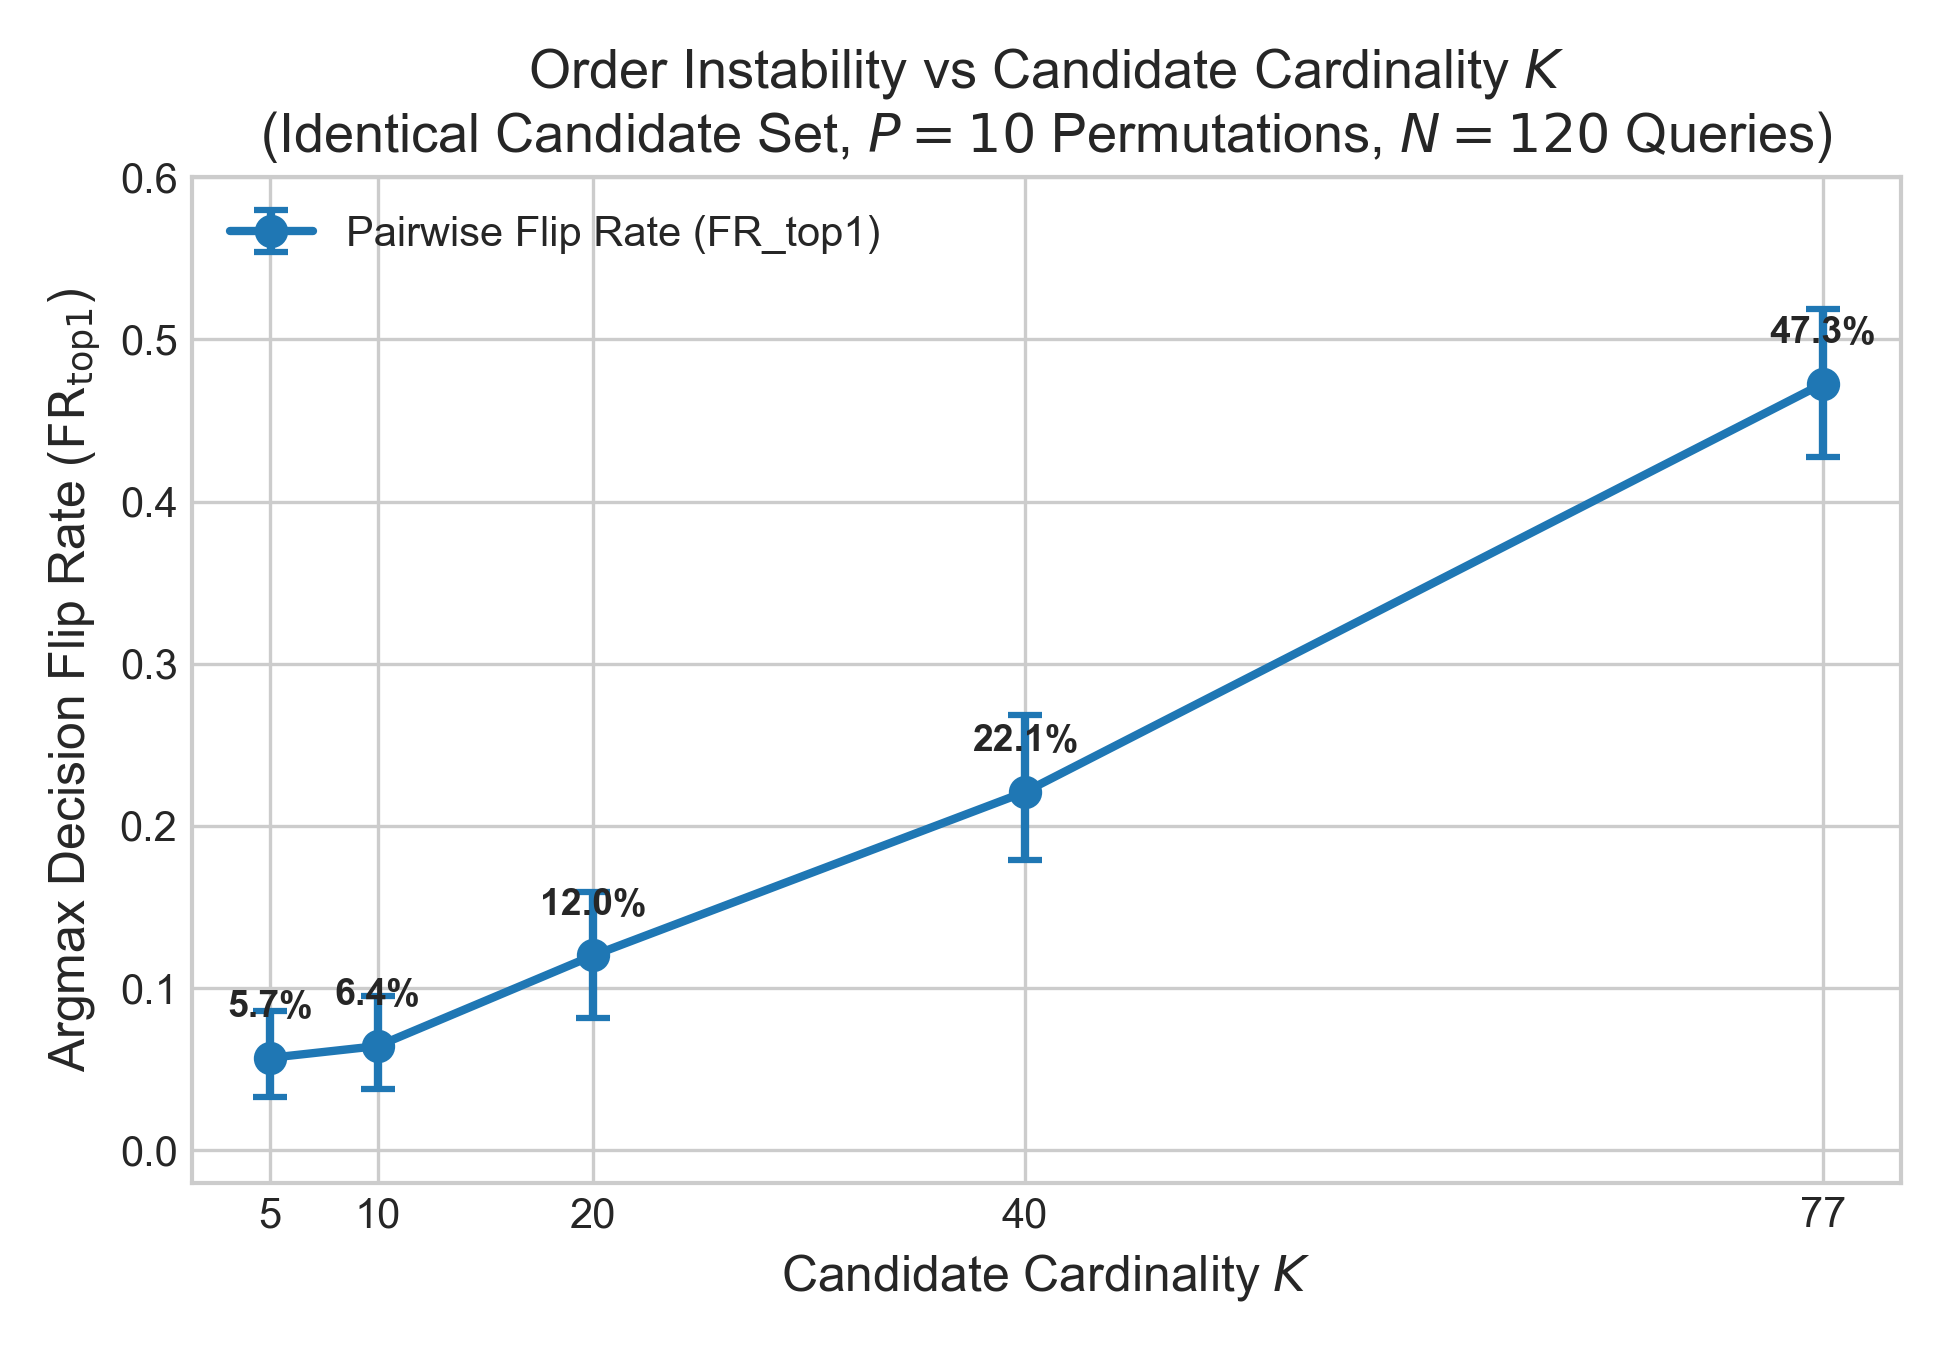
\includegraphics[width=\textwidth]{figures/fig1_cardinality_vs_instability.png}
    \caption{Argmax decision flip rate ($\mathrm{FR}_{\mathrm{top1}}$) scaling.}
    \label{fig:cardinality_instability}
\end{subfigure}
\hfill
\begin{subfigure}[b]{0.48\textwidth}
    \centering
    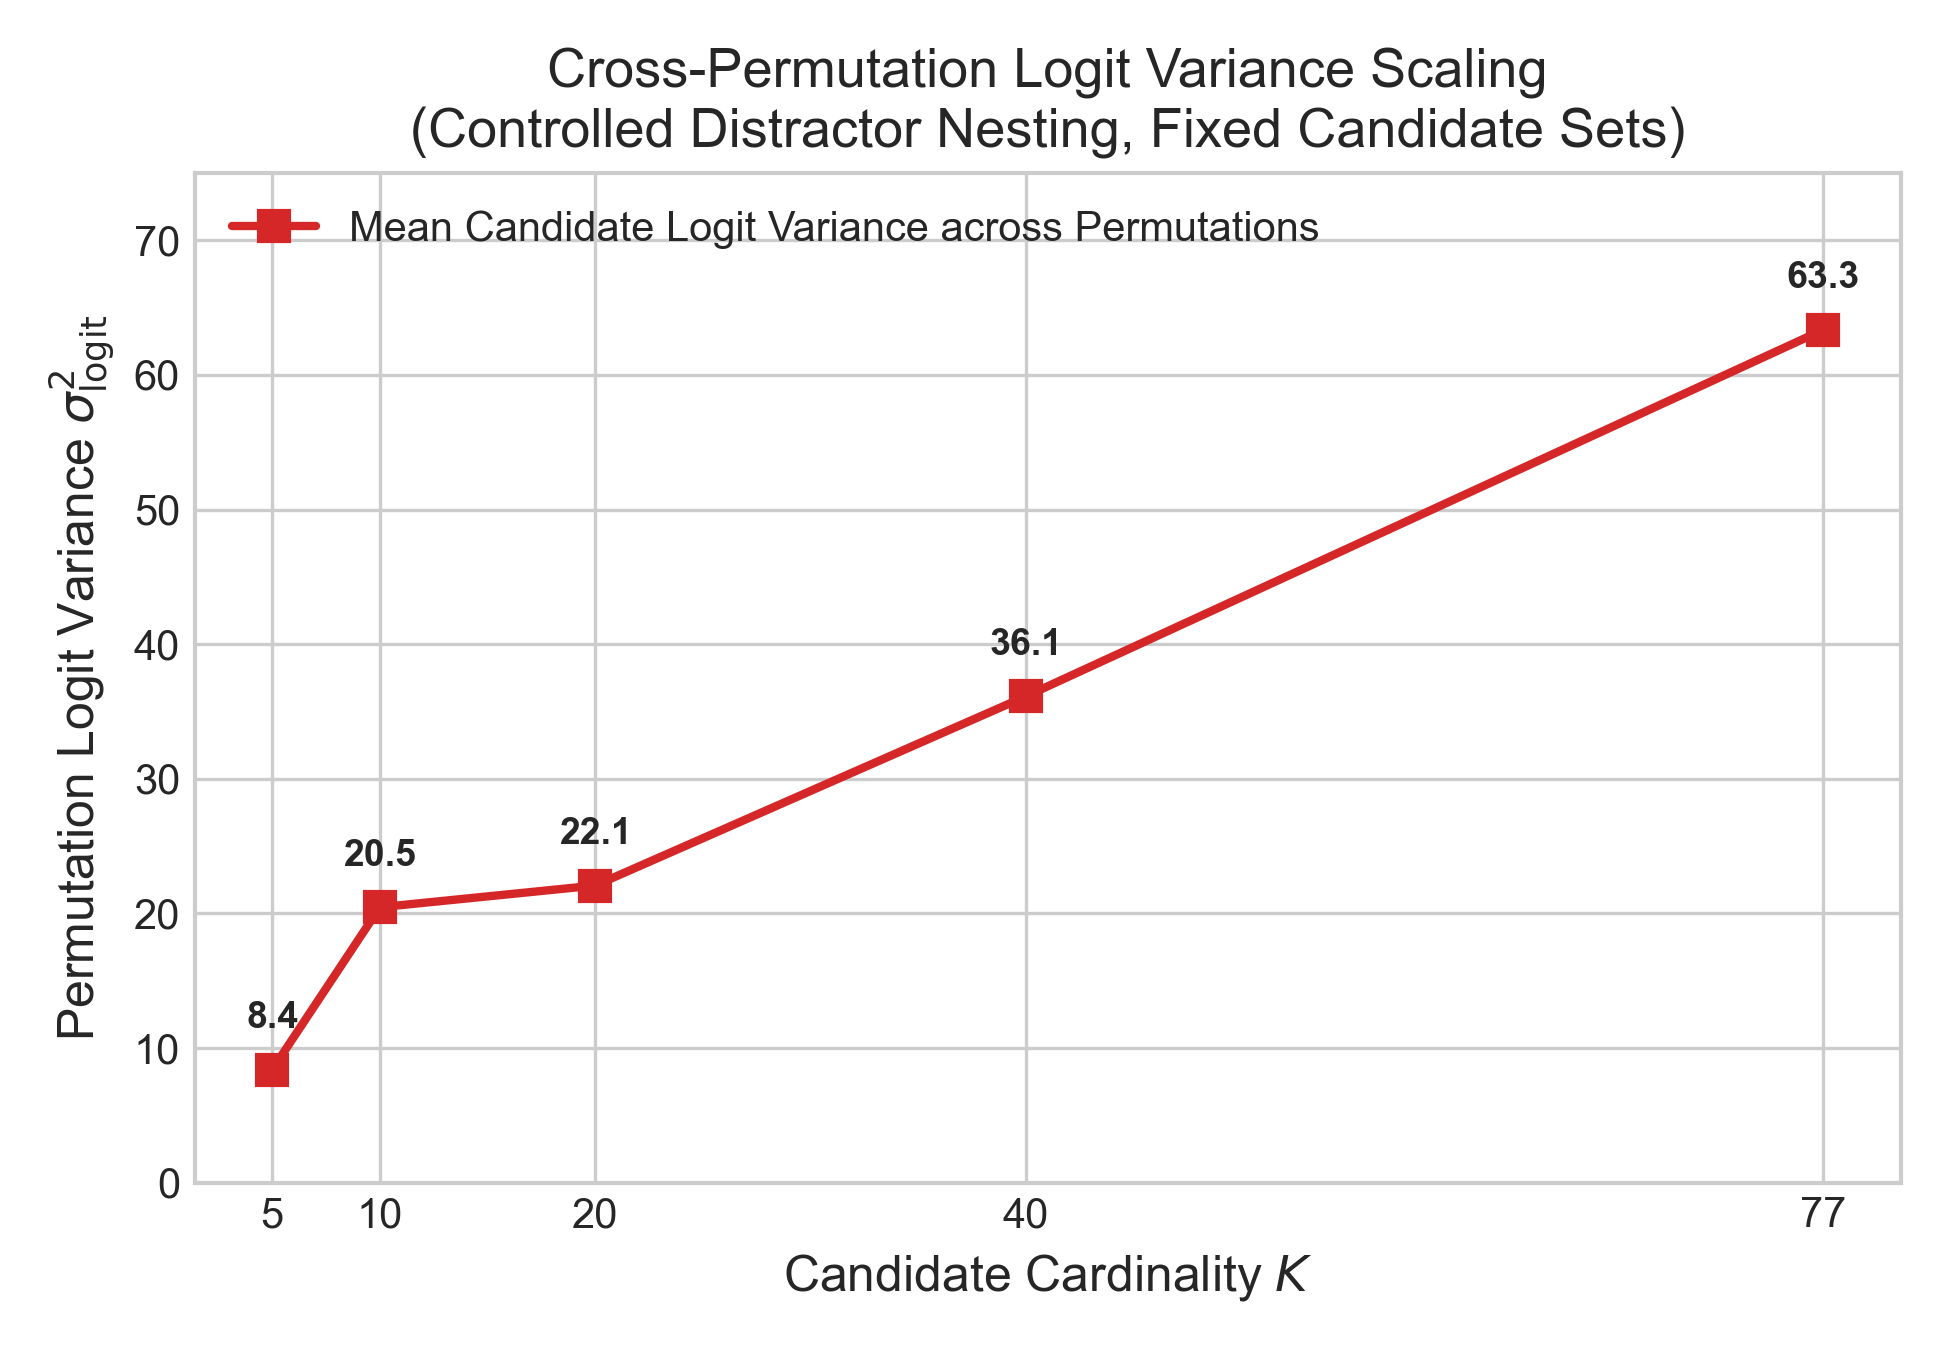
\includegraphics[width=\textwidth]{figures/fig2_cardinality_vs_logit_variance.png}
    \caption{Mean cross-permutation logit variance ($\sigma^2_{\mathrm{logit}}$).}
    \label{fig:logit_variance}
\end{subfigure}
\caption{\textbf{Candidate Cardinality Scaling.} (a) Pairwise decision flip rate $\mathrm{FR}_{\mathrm{top1}}$ strongly increases as candidate cardinality $K$ expands. (b) Mean candidate logit variance across permutations expands by $7.5\times$ ($8.40 \to 63.34$), driven by sequence-length attentional dilution.}
\label{fig:cardinality_scaling}
\end{figure}

This instability is accompanied by a severe expansion in cross-permutation logit volatility. As shown in Figure~\ref{fig:logit_variance}, the mean variance of candidate log-probabilities across permutations increases by $7.5\times$, scaling from $8.40$ at $K=5$ to $63.34$ at $K=77$. As sequence length expands from 60 tokens to over 450 tokens, self-attention entropy distributes over a wider context, increasing marker hidden state variance.

\subsection{The Canonical Ordering Counterfactual}

A common engineering approach to non-deterministic serialization is canonicalization (e.g., sorting candidates alphabetically by label string). Under repeated execution, `B1\_Alpha' achieves perfect repeatability ($\mathrm{FR}_{\mathrm{top1}} \equiv 0.0\%$), giving the illusion of invariance.

\begin{figure}[H]
\centering
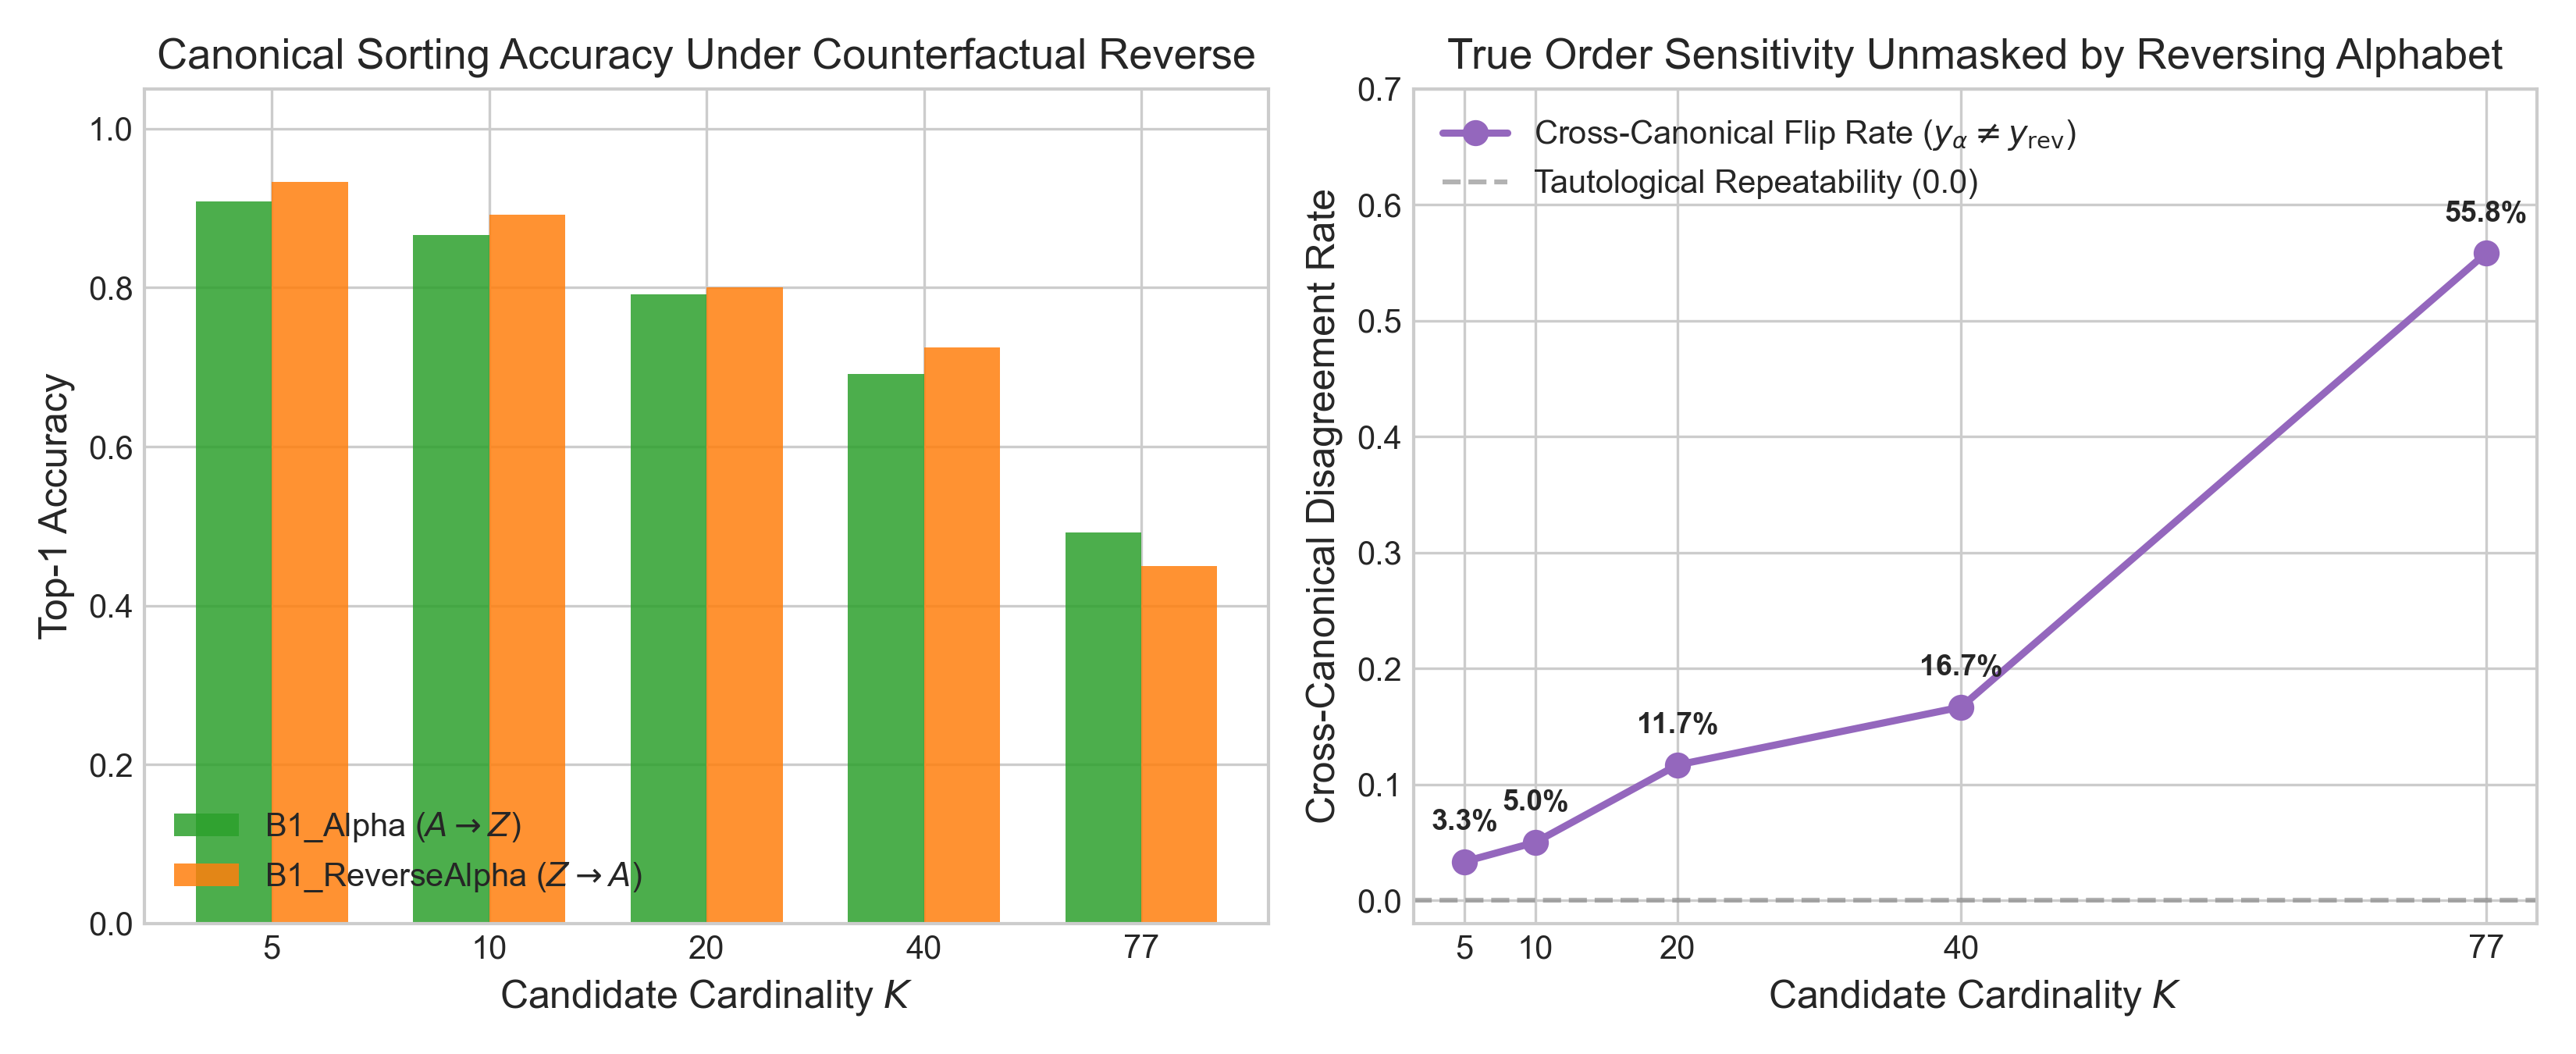
\includegraphics[width=0.88\textwidth]{figures/fig3_canonical_counterfactual.png}
\caption{\textbf{Canonical Counterfactual Analysis.} (Left) Classification accuracy under alphabetical ($A \to Z$) versus reverse alphabetical ($Z \to A$) candidate sorting across cardinalities. (Right) Cross-canonical disagreement rate reaches $55.83\%$ at $K=77$, demonstrating that canonical sorting conceals rather than eliminates underlying positional exposure bias.}
\label{fig:canonical_counterfactual}
\end{figure}

To test whether alphabetical sorting resolves true positional sensitivity, we evaluate the counterfactual reverse-alphabetical ordering (`B1\_ReverseAlpha', $Z \to A$). As depicted in Figure~\ref{fig:canonical_counterfactual}, the cross-canonical flip rate increases from $3.33\%$ [0.8\%, 6.7\%] at $K=5$ to $55.83\%$ [47.5\%, 65.0\%] at $K=77$. At $K=77$, in more than half of all queries, reversing candidate string order alters the model's top-1 classification. Canonicalization does not restore permutation invariance; it merely locks the decision boundary into a static positional bias that systematically favors early-alphabet tokens.

\subsection{Random Marginalization Scaling}

Averaging softmax output probabilities over $M \in \{1, 2, 3, 5\}$ random permutations monotonically reduces residual decision instability. At $K=77$, residual flip rate decreases from $47.28\%$ at $M=1$ down to $38.06\%$ ($M=2$), $34.72\%$ ($M=3$), and $25.83\%$ [20.3\%, 32.0\%] at $M=5$ (Figure~\ref{fig:marginalization_scaling}).

\begin{figure}[H]
\centering
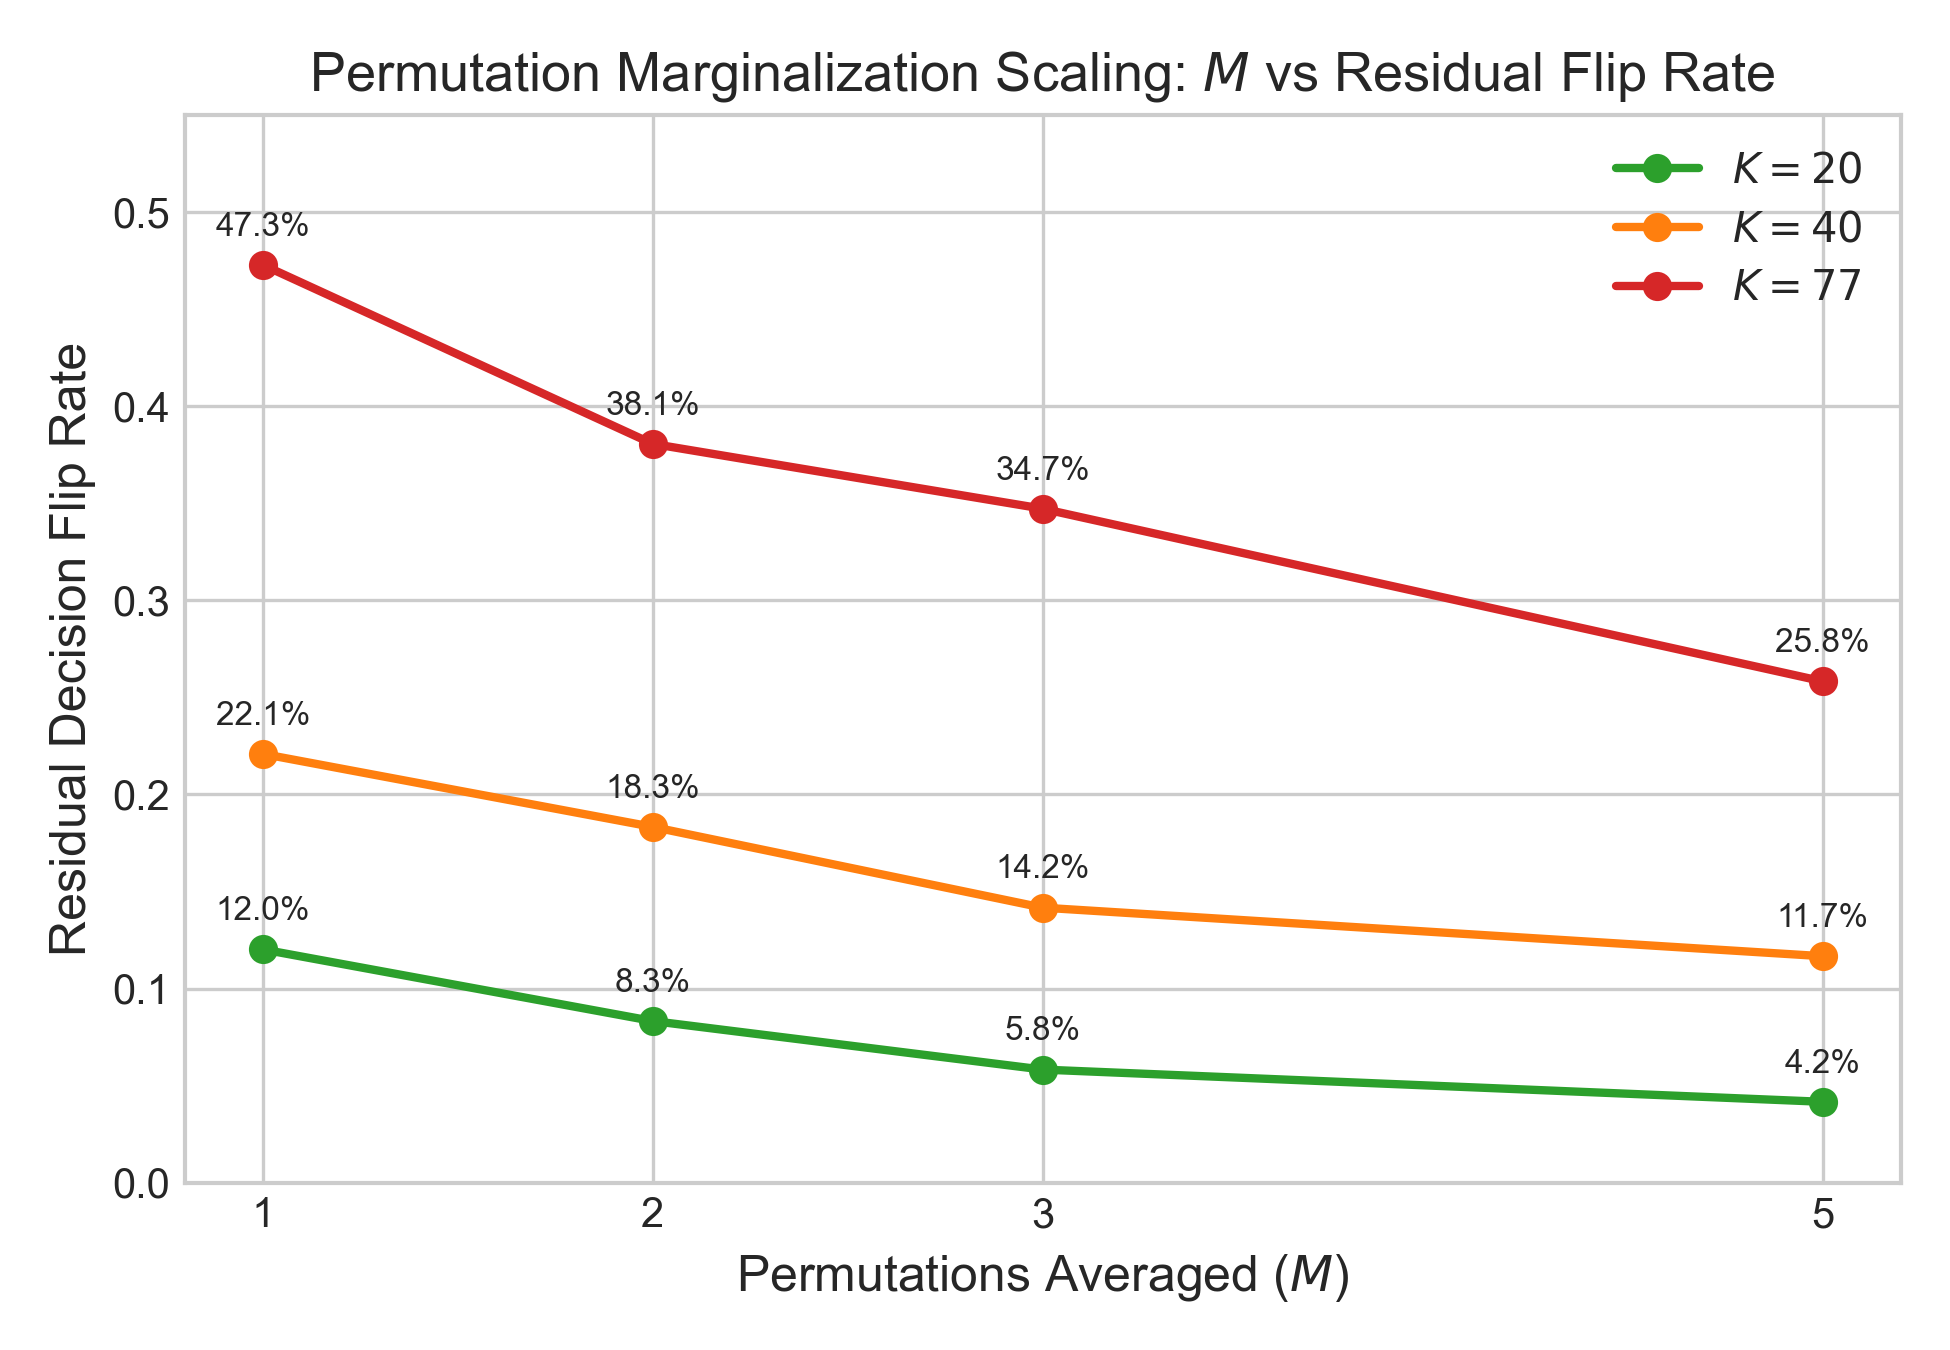
\includegraphics[width=0.65\textwidth]{figures/fig4_marginalization_scaling.png}
\caption{\textbf{Permutation Marginalization Scaling.} Residual decision flip rate decreases monotonically as ensemble passes $M$ increase from 1 to 5 across $K \in \{20, 40, 77\}$.}
\label{fig:marginalization_scaling}
\end{figure}

\subsection{Orthogonal Cyclic Marginalization and Paired Hypothesis Testing}

Deterministic cyclic permutation shifts (`B2\_Cyclic') distribute candidate markers evenly across all sequence positions using orthogonal phase offsets. At equal computational cost ($M=5$ forward passes), cyclic marginalization achieves a residual flip rate of $16.11\%$ [11.9\%, 20.6\%] at $K=77$, compared to $25.83\%$ [20.3\%, 32.0\%] for random marginalization (Figure~\ref{fig:cyclic_vs_random}). Cyclic shifts provide more uniform positional coverage per forward pass than random uniform sampling.

\begin{figure}[H]
\centering
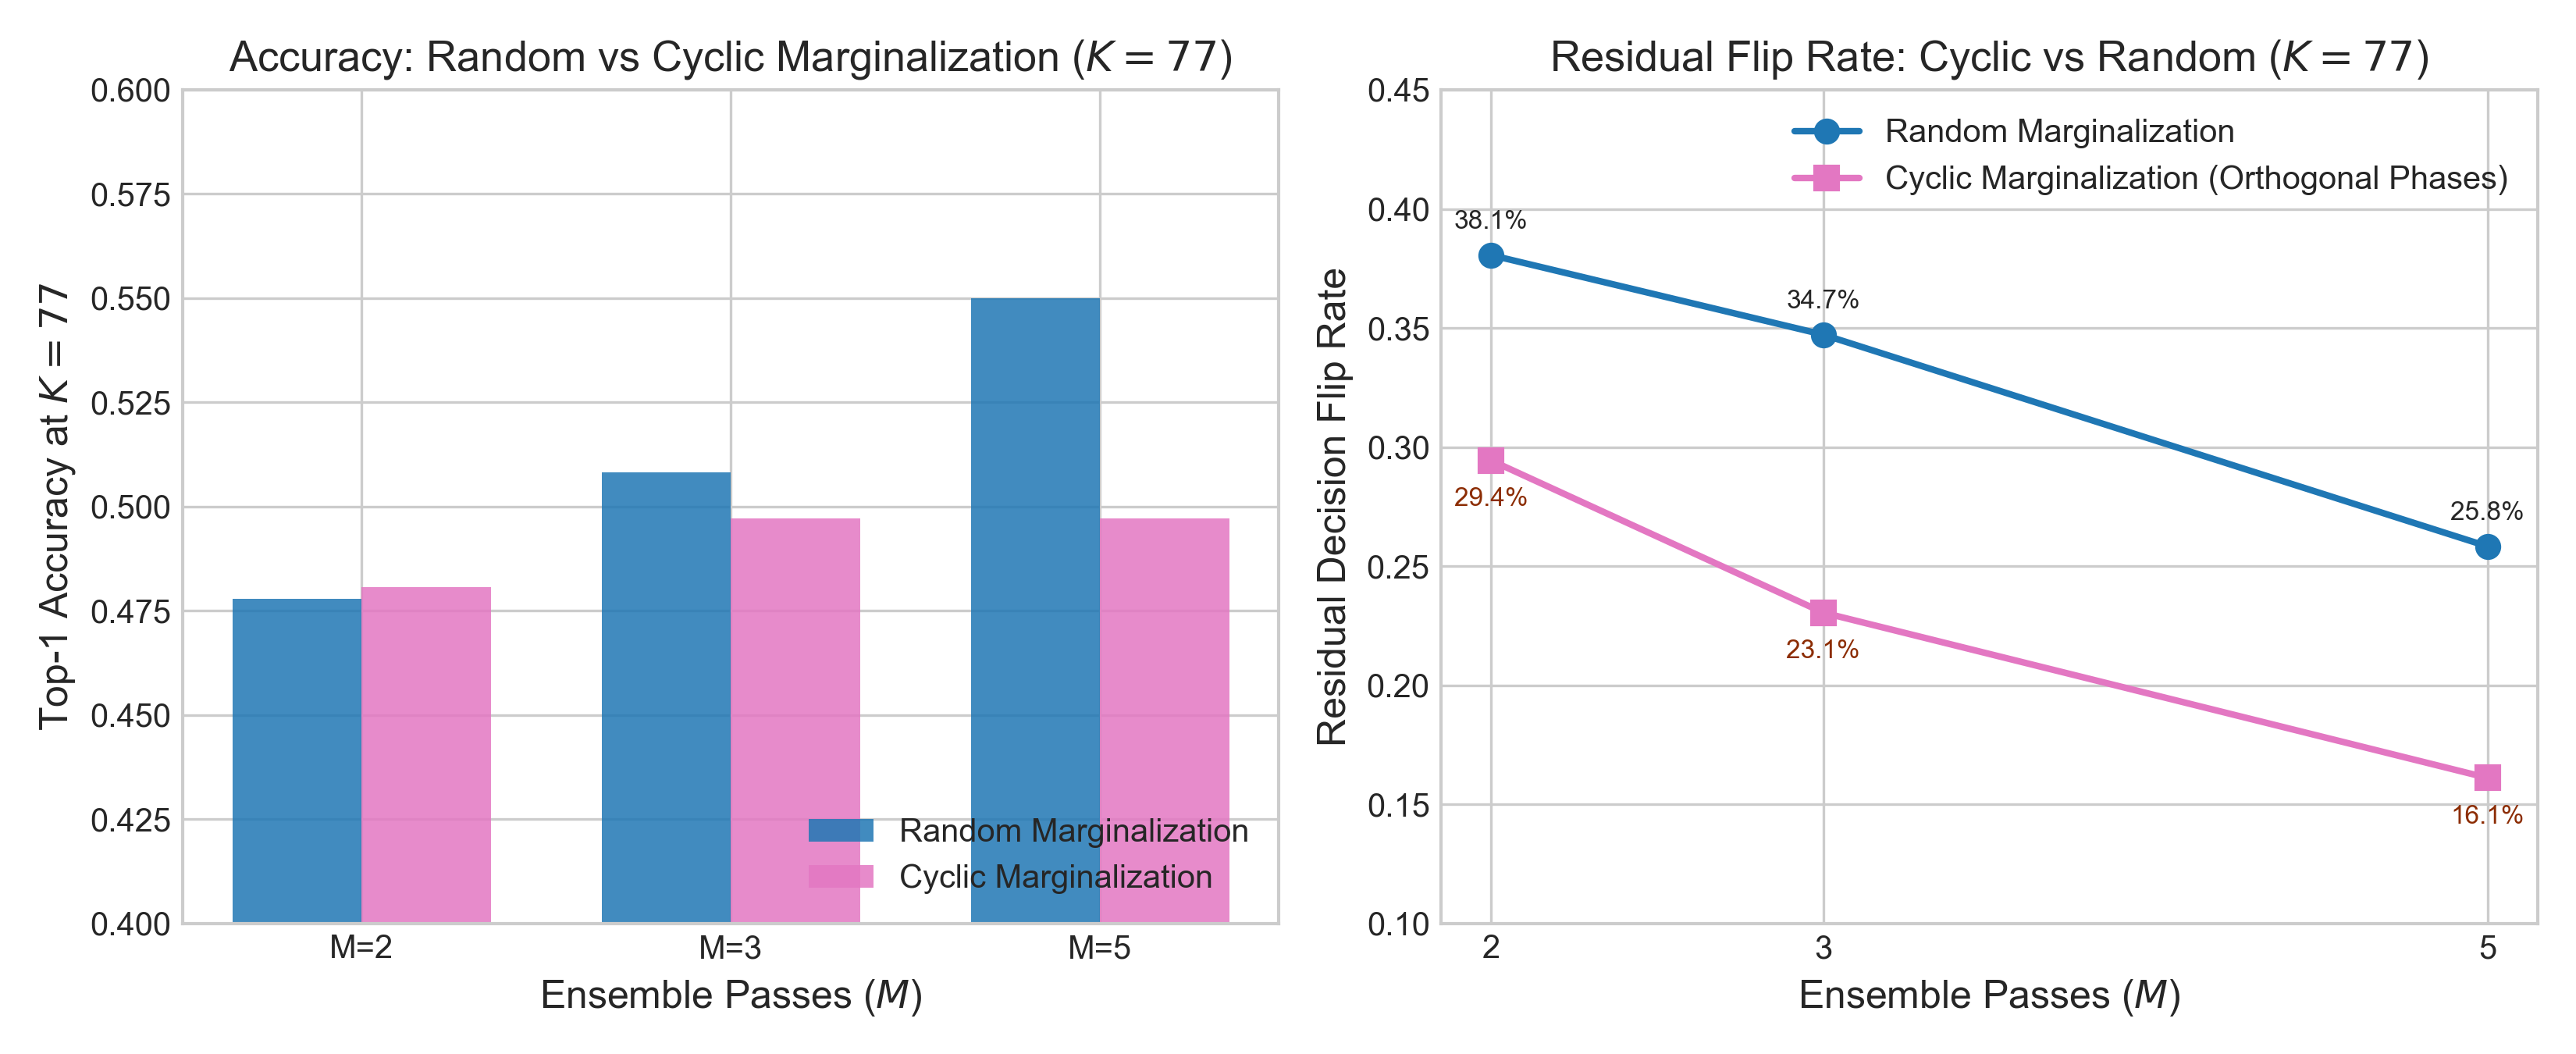
\includegraphics[width=0.88\textwidth]{figures/fig6_cyclic_vs_random.png}
\caption{\textbf{Cyclic versus Random Marginalization at $K=77$.} (Left) Top-1 accuracy comparison across ensemble budgets $M \in \{2, 3, 5\}$. (Right) Residual decision flip rate: cyclic shifts suppress residual instability to $16.11\%$ at $M=5$, compared to $25.83\%$ for random marginalization.}
\label{fig:cyclic_vs_random}
\end{figure}

Across all 45 pre-specified paired comparisons against `B0\_Native' under Benjamini-Hochberg False Discovery Rate control ($q=0.05$), exactly \textbf{one comparison achieved statistical significance}:
\begin{itemize}
    \item \textbf{`B2\_Cyclic\_M5' at $K=40$:} Achieved $70.83\%$ accuracy versus $61.67\%$ for `B0\_Native' ($+9.17$ percentage points, 11 discordant gains, 0 losses, unadjusted two-sided exact McNemar $p = 0.0009765625$, BH-adjusted $p = 0.04395$).
\end{itemize}

At $K=77$, although `Rand\_Marg\_M5' observed an apparent accuracy gain of $+12.78$ percentage points ($55.00\%$ vs $42.22\%$, 27 gains, 11 losses, unadjusted $p=0.0145$), this difference \textbf{failed FDR-adjusted statistical significance} (BH-adjusted $p=1.0000$). With $N=120$ queries and binary outcomes, query-level variance precludes declaring $K=77$ accuracy gains statistically significant under rigorous multiple-testing control. Selected hypothesis test comparisons are summarized in Table~\ref{tab:significance_summary}.

\begin{table}[H]
\centering
\small
\caption{\textbf{Paired Hypothesis Tests vs B0\_Native (Selected Comparisons).} Two-sided exact McNemar tests on discordant classification pairs with Benjamini-Hochberg FDR adjustments ($q=0.05$).}
\label{tab:significance_summary}
\begin{tabular}{r l r c c c c}
\toprule
$K$ & Method & $\Delta$ Accuracy & Gains / Losses & Unadjusted $p$ & BH-Adjusted $p$ & FDR Sig \\
\midrule
5  & B1\_Alpha     & $-1.67\%$ & 1 / 3  & 0.6250   & 1.0000 & No \\
5  & Rand\_Marg\_M5 & $0.00\%$  & 3 / 3  & 1.0000   & 1.0000 & No \\
10 & Rand\_Marg\_M5 & $+0.83\%$ & 1 / 0  & 1.0000   & 1.0000 & No \\
20 & Rand\_Marg\_M5 & $+5.00\%$ & 8 / 2  & 0.1094   & 0.4922 & No \\
40 & B1\_Alpha     & $+7.50\%$ & 10 / 1 & 0.0117   & 0.4922 & No \\
40 & Rand\_Marg\_M5 & $+8.33\%$ & 12 / 2 & 0.0129   & 0.2344 & No \\
\textbf{40} & \textbf{B2\_Cyclic\_M5} & $\mathbf{+9.17\%}$ & \textbf{11 / 0} & $\mathbf{0.00098}$ & $\mathbf{0.04395}$ & \textbf{Yes} ($*$) \\
77 & B1\_Alpha     & $+6.94\%$ & 20 / 12 & 0.2153   & 1.0000 & No \\
77 & B2\_Cyclic\_M5 & $+7.50\%$ & 22 / 13 & 0.1755   & 1.0000 & No \\
77 & Rand\_Marg\_M5 & $+12.78\%$ & 27 / 11 & 0.0145   & 1.0000 & No \\
\bottomrule
\end{tabular}
\end{table}

\subsection{Probability Calibration and ECE Dynamics}

As candidate cardinality expands, single-pass models exhibit severe miscalibration: Expected Calibration Error at $K=77$ reaches $0.3700$ [0.30, 0.45] for `B0\_Native' and $0.3857$ [0.31, 0.47] for `B0\_Random'. Inference-time marginalization provides substantial calibration benefits: at $K=77$, `Rand\_Marg\_M5' reduces ECE to $0.0960$ [0.09, 0.20], and `B2\_Cyclic\_M5' reduces ECE to $0.1619$ [0.13, 0.26]. Averaging probability vectors across permutations dampens extreme, overconfident probability spikes.

\subsection{Query-Level Instability Heterogeneity and Pareto Frontier}

Order instability is not distributed uniformly across queries. As illustrated in Figure~\ref{fig:query_heterogeneity}, $55.0\%$ of queries at $K=77$ experience an argmax flip rate $\mathrm{FR}_{\mathrm{top1}} \ge 50\%$, while a minority of queries remain stable. Query instability exhibits a strong negative Pearson correlation with model confidence:
\begin{equation}
r = -0.4926 \quad (p = 1.09 \times 10^{-8}).
\end{equation}
Queries with high predictive margin between the top-1 and top-2 candidates are resilient to serialization perturbations, whereas queries near decision boundaries fluctuate extensively under sequence reordering.

\begin{figure}[H]
\centering
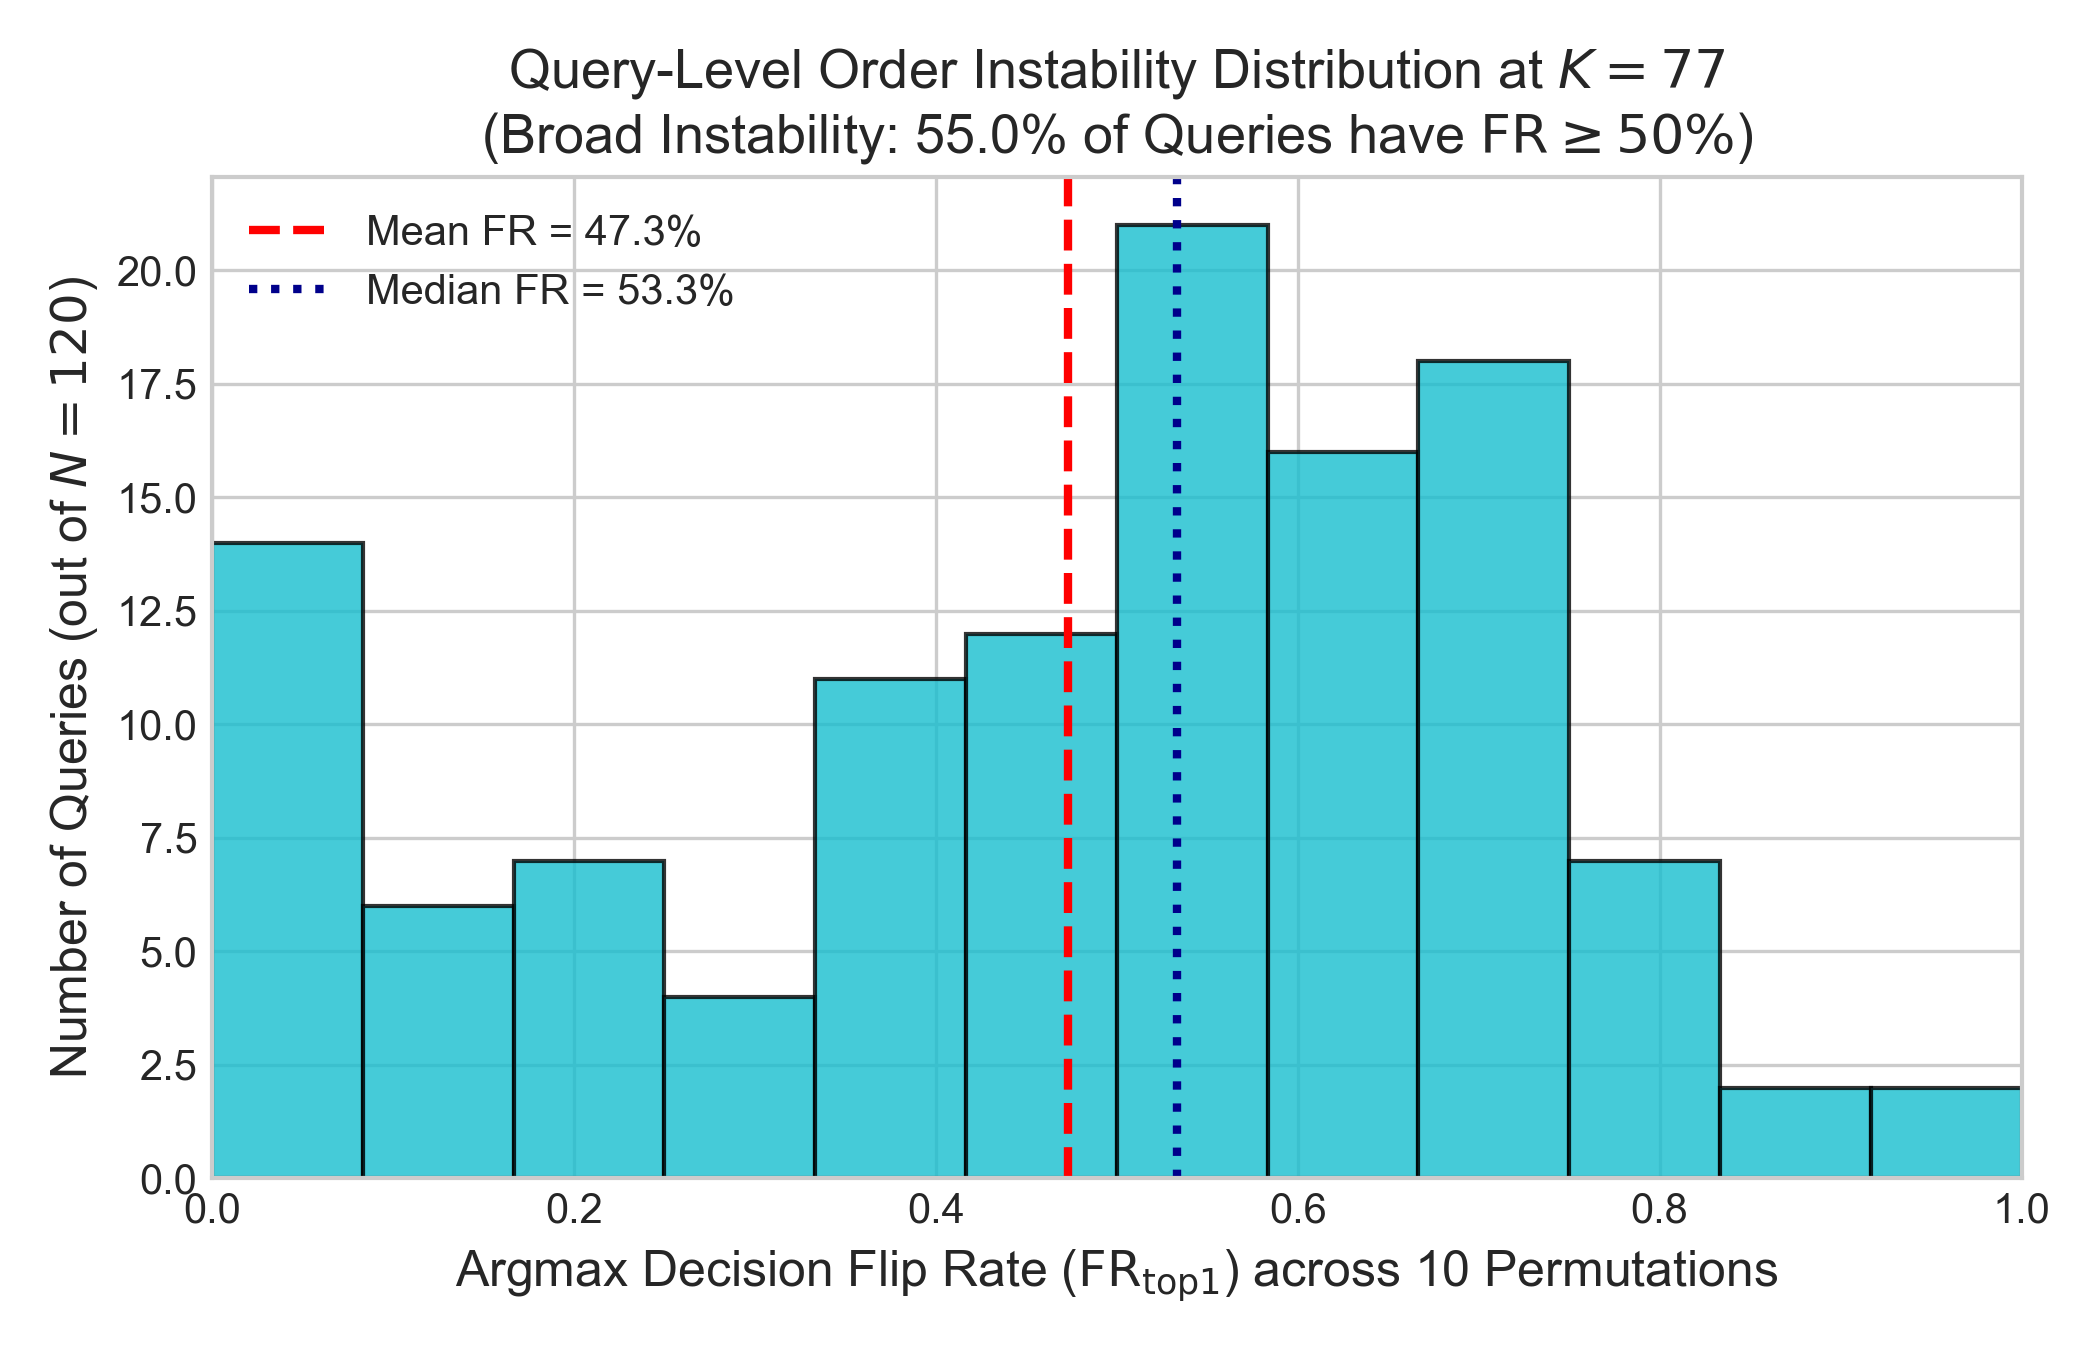
\includegraphics[width=0.68\textwidth]{figures/fig7_k77_query_heterogeneity.png}
\caption{\textbf{Query-Level Instability Distribution at $K=77$.} Distribution of per-query argmax flip rate across 10 random permutations. Over $55.0\%$ of queries experience $\mathrm{FR} \ge 50\%$. Instability is strongly negatively correlated with prediction confidence ($r = -0.4926, p = 1.09 \times 10^{-8}$).}
\label{fig:query_heterogeneity}
\end{figure}

Figure~\ref{fig:pareto_frontier} and Table~\ref{tab:k77_detailed} illustrate the operational trade-offs across Accuracy ($\uparrow$), p50 Latency ($\downarrow$), and within-method Instability ($\downarrow$, measured by $\mathrm{FR}_{\mathrm{top1}}$).

\begin{figure}[H]
\centering
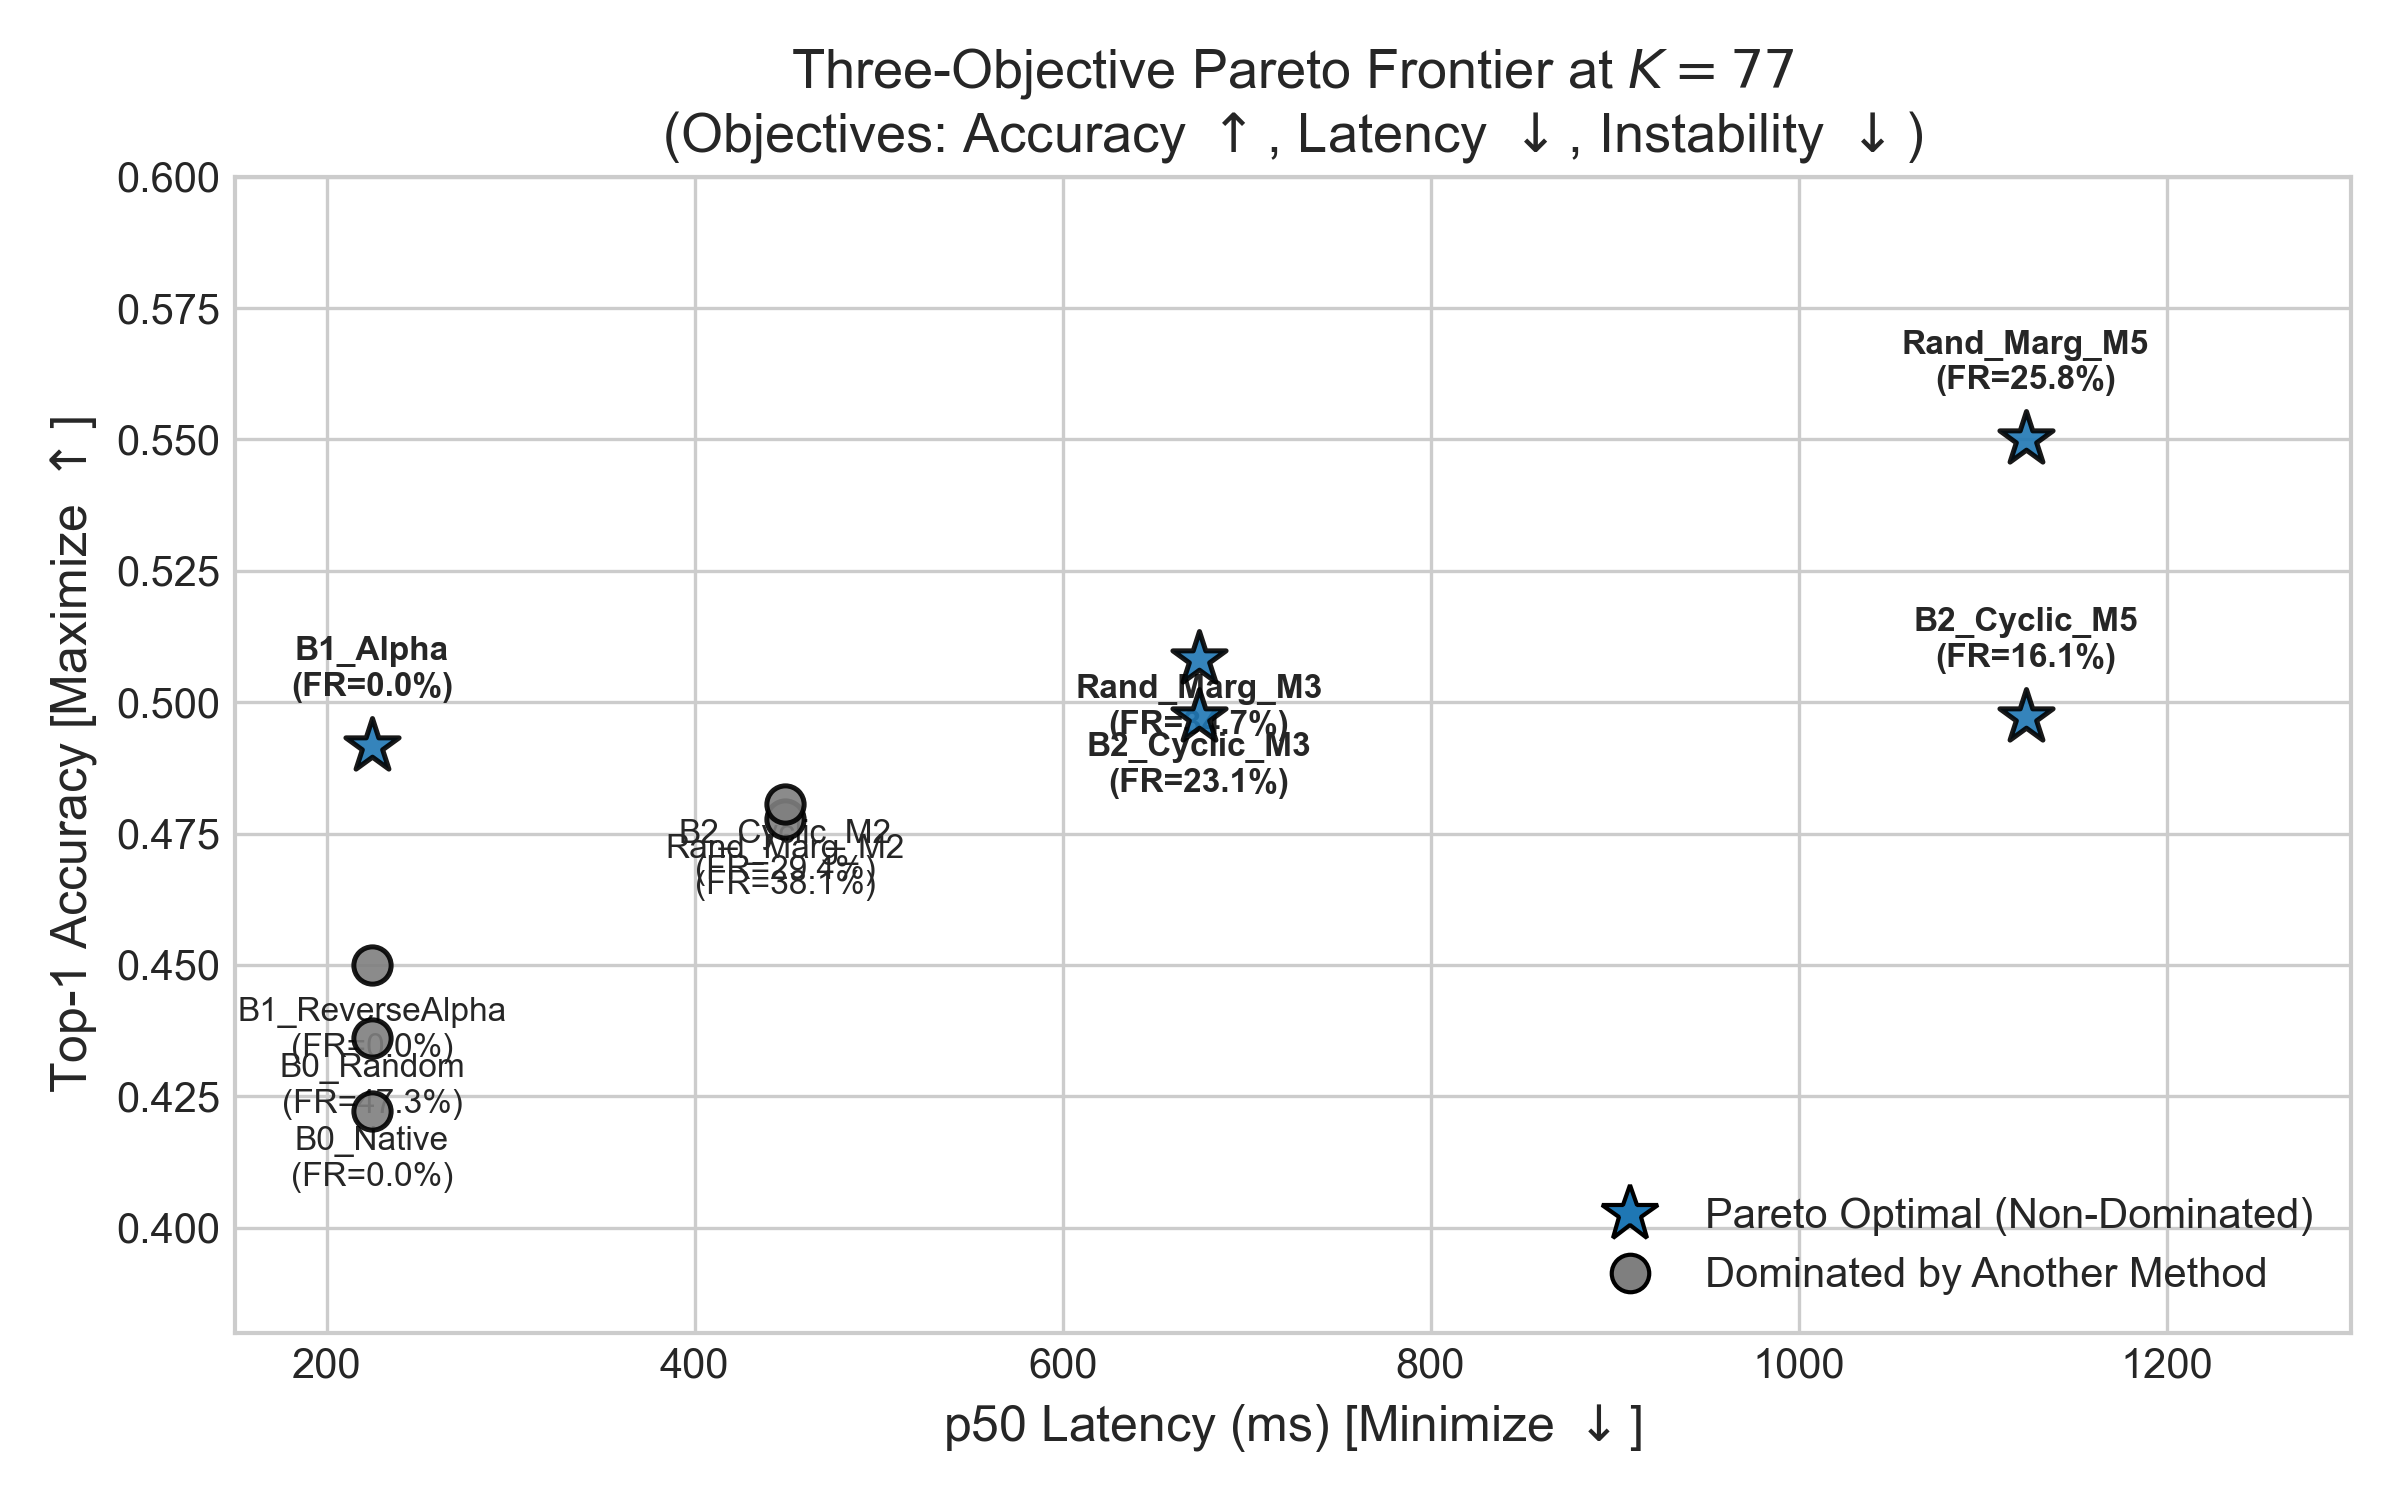
\includegraphics[width=0.75\textwidth]{figures/fig5_pareto_frontier_k77.png}
\caption{\textbf{Three-Objective Pareto Frontier at $K=77$.} Evaluating Accuracy ($\uparrow$), Latency ($\downarrow$), and within-method Instability ($\downarrow$, $\mathrm{FR}_{\mathrm{top1}}$). Non-dominated methods represent Pareto-efficient operating points: `B1\_Alpha' minimizes latency with $0\%$ rerun variance (at the cost of $55.8\%$ cross-canonical exposure bias); `Rand\_Marg\_M5' achieves highest accuracy ($55.0\%$); `B2\_Cyclic\_M5' minimizes residual flip rate ($16.1\%$) among multi-pass methods.}
\label{fig:pareto_frontier}
\end{figure}

\begin{table}[H]
\centering
\small
\caption{\textbf{Detailed Results at Maximum Cardinality ($K=77$).} Evaluated across $N=120$ queries and three base orderings. $\mathrm{FR}_{\mathrm{top1}}$ measures within-method rerun volatility; $\text{Cross-Flip}$ measures counterfactual $A \to Z$ vs $Z \to A$ disagreement.}
\label{tab:k77_detailed}
\resizebox{\columnwidth}{!}{%
\begin{tabular}{l c c c c r c}
\toprule
Method & Accuracy [95\% CI] & ECE [95\% CI] & $\text{FR}_{\text{top1}}$ & Cross-Flip & Latency & Pareto Status \\
\midrule
\textbf{B0\_Native}       & 0.422 [0.34, 0.50] & 0.370 [0.30, 0.45] & 0.000 & --    & 224.7 ms & Dominated \\
\textbf{B0\_Random}       & 0.436 [0.36, 0.51] & 0.386 [0.31, 0.47] & 0.473 & --    & 224.7 ms & Dominated \\
\textbf{B1\_Alpha}        & 0.492 [0.40, 0.58] & 0.334 [0.27, 0.43] & 0.000 & 0.558 & 224.7 ms & \textbf{Non-dominated} \\
\textbf{B1\_ReverseAlpha} & 0.450 [0.37, 0.53] & 0.370 [0.30, 0.46] & 0.000 & 0.558 & 224.7 ms & Dominated \\
\textbf{Rand\_Marg\_M2}   & 0.478 [0.40, 0.55] & 0.202 [0.16, 0.31] & 0.381 & --    & 449.4 ms & Dominated \\
\textbf{Rand\_Marg\_M3}   & 0.508 [0.43, 0.59] & 0.204 [0.16, 0.29] & 0.347 & --    & 674.0 ms & \textbf{Non-dominated} \\
\textbf{Rand\_Marg\_M5}   & \textbf{0.550 [0.47, 0.62]} & \textbf{0.096 [0.09, 0.20]} & 0.258 & -- & 1123.4 ms & \textbf{Non-dominated} \\
\textbf{B2\_Cyclic\_M2}   & 0.481 [0.41, 0.56] & 0.218 [0.16, 0.31] & 0.294 & --    & 449.4 ms & Dominated \\
\textbf{B2\_Cyclic\_M3}   & 0.497 [0.42, 0.57] & 0.147 [0.11, 0.24] & 0.231 & --    & 674.0 ms & \textbf{Non-dominated} \\
\textbf{B2\_Cyclic\_M5}   & 0.497 [0.42, 0.58] & 0.162 [0.13, 0.26] & \textbf{0.161} & -- & 1123.4 ms & \textbf{Non-dominated} \\
\bottomrule
\end{tabular}%
}
\end{table}

\section{Important Negative Replication Result}

In preliminary exploratory benchmarking ($N=40, S=1$ base sequence), an anomalous accuracy of \textbf{$65.0\%$} was observed for cyclic shifts ($M=2$) at $K=77$, leading to an initial conjecture that cyclic shifts dramatically improve classification accuracy at full cardinality.

Under our pre-specified replication protocol ($N=120$ unique queries, stratified sampling, $S=3$ independently seeded base candidate sequences `[alphabetical, 7701, 7702]'):
\begin{itemize}
    \item Replicated `B2\_Cyclic\_M2' accuracy is \textbf{$48.06\%$ [39.7\%, 55.6\%]}, statistically indistinguishable from random marginalization ($47.78\%$).
    \item Replicated `B2\_Cyclic\_M5' accuracy is \textbf{$49.72\%$ [41.7\%, 57.2\%]}.
\end{itemize}
This negative result is documented as an integral empirical finding. At high candidate cardinality ($K=77$), small sample sizes ($N=40$) combined with anchoring to a single arbitrary base candidate sequence produce false-positive accuracy spikes. Controlled multi-seed replication corrected this exploratory artifact.

\section{Discussion}

\paragraph{Architecture-Induced Order Sensitivity.}
In contrast to bi-encoders that score candidates independently, multi-candidate concatenation introduces cross-candidate attentional competition. Because token representations are coupled through bidirectional self-attention and positional embeddings, candidate order acts as a hidden nuisance parameter.

\paragraph{Canonicalization vs.\ Permutation Invariance.}
Alphabetical canonicalization is widely used to enforce deterministic model outputs in production pipelines. Our counterfactual analysis demonstrates that canonicalization merely fixes a single arbitrary permutation, concealing underlying order sensitivity. If label strings are translated, renamed, or prefixed, decisions flip on $55.83\%$ of queries at $K=77$.

\paragraph{Inference-Time Marginalization.}
Permutation marginalization provides an inference-time solution without requiring architectural retraining. At $M=5$, orthogonal cyclic shifts reduce residual decision flip rate to $16.11\%$ while reducing Expected Calibration Error from $0.3857$ to $0.1619$. However, marginalization incurs an $M\times$ latency overhead, establishing a clear trade-off between latency and decision stability.

\section{Limitations}

\begin{enumerate}
    \item \textbf{Single Backbone and Checkpoint:} All evaluations were conducted on the \nolinkurl{convaiinnovations/laya} model checkpoint (RoBERTa-based bidirectional encoder). While the marker concatenation pattern is general, the exact magnitude of instability may vary across backbones and pretraining objectives.
    \item \textbf{Domain Specialization:} Our study evaluates the Banking77 benchmark. Intent classification provides clean distractor subsets, but semantic dynamics in open-domain tool routing may differ.
    \item \textbf{Inference-Time Scope:} We investigate post-training inference-time interventions; we do not evaluate training-time data augmentation (e.g., training with randomized permutations) or permutation-invariant pooling layers.
    \item \textbf{Statistical Power at $K=77$ ($N=120$):} Detecting a $+5\%$ to $+10\%$ accuracy gain under Benjamini-Hochberg FDR control across 45 comparisons requires $N \ge 350$ queries due to binary classification variance.
\end{enumerate}

\section{Conclusion}

Candidate presentation order induces substantial decision instability in non-autoregressive multi-candidate transformers, scaling from $5.70\%$ at $K=5$ to $47.28\%$ at $K=77$. Canonical alphabetical sorting achieves deterministic repeatability but conceals a $55.83\%$ counterfactual cross-order disagreement rate. Inference-time permutation marginalization systematically suppresses residual instability and improves calibration, with orthogonal cyclic shifts achieving $16.11\%$ residual flip rate at $M=5$. Across 45 pre-specified paired comparisons, cyclic marginalization at $K=40$ achieves the sole statistically significant accuracy improvement ($+9.17$ percentage points, adjusted $p=0.04395$). These findings demonstrate that candidate serialization is an active source of variance in multi-candidate encoders that requires explicit algorithmic marginalization or invariant pooling.

\section{Reproducibility Statement}

To ensure complete scientific reproducibility while strictly maintaining double-blind review integrity, all benchmark execution harnesses, exact candidate configuration manifests, invariant unit test suites, and raw per-query evaluation CSVs are provided in the accompanying anonymized Supplementary Material package. Upon completion of the peer review process, the full public version-controlled repository and permanent Zenodo digital object identifier (DOI) will be linked in the camera-ready version.

\subsubsection*{Broader Impact Statement}

This investigation systematically analyzes candidate presentation order as an unmodelled nuisance variable in non-autoregressive multi-candidate transformers.
\paragraph{Positive Impacts.} Identifying order instability and providing inference-time marginalization algorithms improves the reliability, determinism, and calibration of automated classification and tool-routing pipelines. By demonstrating that alphabetical canonicalization conceals rather than eliminates positional exposure bias, this study provides actionable diagnostic protocols for practitioners deploying multi-candidate encoders in sensitive conversational domains (such as banking and financial services).
\paragraph{Potential Negative Impacts and Automation Risks.} A potential risk is that practitioners might misinterpret inference-time marginalization as a complete guarantee of permutation invariance. Although cyclic marginalization substantially reduces residual decision flips (suppressing flip rates to $16.11\%$ at $M=5$), residual instability remains non-zero. Relying uncritically on marginalization in high-stakes automated action execution without threshold-based human oversight could perpetuate unexpected decision shifts.
\paragraph{Mitigations.} We explicitly document the exact residual flip rates, delineate Pareto operating trade-offs, emphasize statistical power boundaries, and package all evaluation artifacts into reproducible verification suites to prevent premature or misleading claims of robustness.

\bibliography{references}
\bibliographystyle{tmlr}

\appendix
\section{Supplementary Experimental Details and Invariant Protocols}

\subsection{Distractor Sampling Hierarchy}
For each query $q$ with label $y^*$, the candidate set $\mathcal{C}_K(q)$ satisfies:
\begin{equation}
\mathcal{C}_5(q) \subset \mathcal{C}_{10}(q) \subset \mathcal{C}_{20}(q) \subset \mathcal{C}_{40}(q) \subset \mathcal{C}_{77}(q) = \mathcal{C}_{\text{all}}.
\end{equation}
The ground-truth label $y^*$ is always present in $\mathcal{C}_K(q)$. Distractors are selected using deterministic pseudo-random sampling seeded by the query ID, ensuring zero confounding from stochastic distractor replacement.

\subsection{Deterministic Invariant Verification Suite}
All experimental outputs are verified against six deterministic mathematical invariants:
\begin{enumerate}
    \item \textbf{Ground-Truth Containment:} $y^* \in \mathcal{C}_K(q)$ for all $K \in \{5, 10, 20, 40, 77\}$.
    \item \textbf{Candidate Cardinality Invariant:} $|\mathcal{C}_K(q)| = K$ exactly.
    \item \textbf{Nested Distractor Invariant:} $\mathcal{C}_K(q) \subset \mathcal{C}_{K'}(q)$ for all $K < K'$.
    \item \textbf{Canonical Sorting Invariant:} $\mathrm{FR}_{\mathrm{top1}}(\text{B1\_Alpha}) \equiv 0.0\%$.
    \item \textbf{Cross-Canonical Separation:} $\mathrm{CrossCanonicalFlip}$ is distinct from within-method $\mathrm{FR}_{\mathrm{top1}}$.
    \item \textbf{Probability Calibration Bound:} $\mathrm{ECE} \in [0, 1]$ and all confidence intervals satisfy $\text{Lo} \le \text{Estimate} \le \text{Hi}$.
\end{enumerate}

\end{document}
